\documentclass[12pt,twoside,notitlepage]{report}
\newcommand{\fxch}{FixCache}
\usepackage{a4}
\usepackage{verbatim}
\usepackage{amsmath}
\usepackage{color}
\usepackage[T1]{fontenc}
\usepackage[dvipsnames]{xcolor}
\usepackage{listings}
\usepackage{enumitem}
\usepackage[boxed]{algorithm2e}
\usepackage{fixltx2e}


\usepackage{graphicx}
\usepackage[labelfont=bf]{caption}
\usepackage{wrapfig}
\usepackage[rightcaption]{sidecap}
\makeatletter
\setlength{\@fptop}{0pt}
\makeatother
\graphicspath{ {figs/} }

\title{Dissertation draft (1st and last chapter ommitted)}
\author{Tamas Sztanka-Toth \\ ts579@cam.ac.uk}
\raggedbottom                           % try to avoid widows and orphans
\sloppy
\clubpenalty1000%
\widowpenalty1000%

\addtolength{\oddsidemargin}{6mm}       % adjust margins
\addtolength{\evensidemargin}{-8mm}

\renewcommand{\baselinestretch}{1.1}    % adjust line spacing to make
                                        % more readable

\begin{document}

\lstset{language=bash, tabsize=4, backgroundcolor=\color{lightgray}, keywordstyle=\color{black}, frame=single, framesep=10pt, xleftmargin=10pt, xrightmargin=10pt}
\setcounter{page}{1}
\pagenumbering{roman}
\pagestyle{plain}
\bibliographystyle{unsrt}      % just to make sure before the page numbering
                        % is changed



\pagestyle{empty}

\hfill{\LARGE \bf Tamas Sztanka-Toth}

\vspace*{60mm}
\begin{center}
\Huge
{\bf Cached Bug Prediction for Python repositories on GitHub} \\
\vspace*{5mm}
Computer Science Tripos - Part II \\
\vspace*{5mm}
Homerton College \\
\vspace*{5mm}
\today  % today's date
\end{center}

\cleardoublepage

%%%%%%%%%%%%%%%%%%%%%%%%%%%%%%%%%%%%%%%%%%%%%%%%%%%%%%%%%%%%%%%%%%%%%%%%%%%%%%
% Proforma, table of contents and list of figures

\setcounter{page}{1}
\pagenumbering{roman}
\pagestyle{plain}

\chapter*{Proforma}

{\large
\begin{tabular}{ll}
Name:               & \bf Tamas Sztanka-Toth                       \\
College:            & \bf Homerton College                     \\
Project Title:      & \bf Cached Bug Prediction for Python repositories\\ 						& \bf on GitHub \\
Examination:        & \bf Computer Science Tripos - Part II, July 2016        \\
Word Count:         & \bf X\footnotemark[1]				 \\
Project Originator: & Advait Sarkar                \\
Supervisor:         & Advait Sarkar                    \\ 
\end{tabular}
}
\footnotetext[1]{This word count was computed
by {\tt detex diss.tex | tr -cd '0-9A-Za-z $\tt\backslash$n' | wc -w}
}
\stepcounter{footnote}


\section*{Original Aims of the Project}


\section*{Work Completed}

\section*{Special Difficulties}
 
\newpage
\section*{Declaration}

I, Tamas Sztanka-Toth of Homerton College, being a candidate for Part II of the Computer
Science Tripos, hereby declare
that this dissertation and the work described in it are my own work,
unaided except as may be specified below, and that the dissertation
does not contain material that has already been used to any substantial
extent for a comparable purpose.

\bigskip
\leftline{Signed }

\medskip
\leftline{Date }

\cleardoublepage

\tableofcontents

\listoffigures

\newpage
\section*{Acknowledgements}


%%%%%%%%%%%%%%%%%%%%%%%%%%%%%%%%%%%%%%%%%%%%%%%%%%%%%%%%%%%%%%%%%%%%%%%
% now for the chapters

\cleardoublepage        % just to make sure before the page numbering
                        % is changed
\setcounter{page}{1}
\pagenumbering{arabic}
\pagestyle{headings}
\chapter{Introduction}
\cleardoublepage
\chapter{Preparation}
This chapter summarizes the work done before implementation, relevant literature and concepts used by \fxch{} algorithm. It first discusses \fxch{} and it's background; then it describes Git\cite{TorvaldsGit} software management system and how can it be used to implement \fxch{}. Finally, in this chapter we will look at GitPython: a Python library used to acces Git repositories.
\section{Overview of \fxch{} algorithm}
\subsection{History}
\fxch{} is a bug-prediction algorithm implemented in 2007 by researchers at MIT\cite{FixCache}. The original algorithm was implemented for Subversion and CVS, whereas my implementation is for Git. These Source Code Management systems differ in lot of aspects, the key difference between Git and the others, is that Git is distributed, that is it does not require a central `parent` or `master` repository. This means that we do not need a remote server access every time we want to commit a new change, we simply commit them locally, and later we can push those commits to a remote location. This feature speeds up programming, but also it introduces new problems to tackle when one is mining repositories\cite{Git}.

The authors argued in the original paper that after \fxch{} is ran for a repository it will correctly identify some subset of the repositories file-base which subset is said to contain files which are "more likely to have a bug in the future". This dissertation will further explore this proposition, will discuss the best parameter for \fxch{} and in the Evaluation chapter will compare results with the original paper.
\subsection{Abstract view of the algorithm}
The algorithm works as follows:
\begin{enumerate}
	\item Preload the cache with initial items (new-entity locality).
	\item For each commit C in the repository, starting from the first commit:
	\item If the commit is identified as a fixing-commit:
		
	For each file uploaded by that commit, we check if they are in the cache. If a file is in the cache, we record a hit, else we record a miss.
	\item For each file $F$ which were not in the cache, we go back to the commits when the bugs in those files were introduced (say revision $n$), and take some closest files to $F$, at revision $n$ (spacial locality).
	\item We select some subset of new-files and changed-files at C, and put this subset to the cache (new-entity locality and changed-entity locality).
	\item We remove those files from the cache, which were deleted at C (clean-up).
\end{enumerate}

So far, files were only added to the cache. What happens is that the algorithm in the background takes care of cache pollution, and removes files from the cache to make space for new arrivals.
\subsubsection*{Cache-replacement policies}
The algorithm itself is called \fxch{} as it uses a notion of a cache, which stores a subset of files in a repository. Following this logic, the algorithm defines a notion of locality: spacial, temporal, new-entity and changed-entity. We use these localities to put files into the cache, to increase its accuracy. As the number of files in the cache (the cache-size) is fixed, we need to take out files from the cache if the cache is polluted. There exist different cache replacement policies\cite{FixCache}:
\begin{itemize}
\item \textit{Least-recently-used (LRU)}: When removing files from the cache we first remove those which were used least-recently. That is they were added/changed earlier in the commit history.
\item \textit{LRU weighted by number of changes (CHANGE)}: This approach will remove files which were changed the least, as the intuition is that more frequently used files are more bug-prone, so we want to keep them in the cache.
\item \textit{LRU weighted by number of faults}: This is similar to the approach before, the only difference is that instead of removing files with least changes it removes files with least faults.
\end{itemize}
In the implementation itself I have used the LRU cache replacement policy, as it is simple, and there is not significant difference between the different replacement policies\cite{FixCache}\cite{Sadowski}\cite{Bugcache}.
\subsection{Hits, misses and hit rate}
We only look-up the cache at the so-called bug-fixing commits. To flag a commit as a bug-fixing one, we use a set of regular expressions (which are listed in more detail in section \ref{parsing}) and parse the commit message. If a message matches any of our regular expressions, it is a bug-fixing commit (following the idea used in \cite{KimZim}).
Some examples of bug-fixing commit messages\footnote{All examples taken from identified commit-messages of facebook-sdk.git repository, explained later.}:
\begin{itemize}
\item \texttt{Simple json module import. Fixes \#106.}

\item \texttt{bugfix: changed key of id from user to id in the user dict stored in the session}
\item \texttt{Final fix for Python 2.6 tests.}
\item \texttt{PEP8 fixes. Make sure that code is compliant with pep8 1.3.3.}
\end{itemize}

At each bug-fixing commit, for each file involved in that commit, we make a lookup in the cache. If a file is already in the cache, we note a hit. Otherwise we score a miss. Then we define hit-rate, as the ratio of hits over all lookups, that is:
\[
	hitrate = \frac{\#hits}{(\#misses + \#hits)}
\]
Since at each commit we either increase the hit-count or miss-count (or both), the hit-rate itself is a cumulative indicator of how good our algorithm is. 

At each commit, the cache contains both fault and non-faulty files. What is really important in \fxch{}, is that only truly faulty files score hits, so there is a relation between the hit-rate and True-positives (files that are faulty and are in the cache) in the cache itself, that is there is a relation between hit-rate and the number of identified faulty files. Some might argue that this evaluation strategy is poor, as it is not known what is the window of our prediction, that is how early/late will the files in the cache contain bugs. There exists other, more sophisticated evaluations, by other authors such as \cite{Sadowski} and \cite{Bugcache} which look at: examples here....
\subsection{Cache-localities and variables}\label{variables}
As mentioned before there are four different localities when talking about \fxch{}: temporal, spatial, changed-entity and new-entity. 
\subsubsection{Temporal-locality}
As with physical caches, temporal-locality in \fxch{} is used following the idea that files which were used (had a fault) will be used (will have a fault) in the near future. At each bug-fixing commit, we load all the files involved in the cache, regardless of whether we recorded a hit, or miss for them.
\subsubsection{Spatial-locality}
Again, the idea of spatial-locality comes from the world of physical caches: when a file is used (has a fault) it is likely that other files "near" to that file will be used (will have a fault). To define nearness, we first need to define the notion of distance for two files in \fxch{}. Distance is for any two files $f_1$ and $f_2$ at revision/commit $n$ is defined as (following \cite{FixCache}):
\[
	distance(f_1, f_2, n) = \frac{1}{cooccurrence(f_1, f_2, n)}
\]
The $coocurrence(f_1, f_2, n)$ returns an integer: how many times were the files $f_1$ and $f_2$ used (committed) together from revision $0$ to revision $n$.

\textbf{Distance-to-fetch (block-size)}: this parameter (variable) is used to define how many files will be fetched when loading the closest files to a file at revision $n$.

This locality is used every time we have a cache-miss. If a file (say $f_t$) is missed during a bug-fixing commit, we go back to the bug-introducing commit(s) and fetch the closest files to $f_t$ at each bug-introducing commit identified. We can identify the bug-introducing commits using the SZZ algorithm\cite{SZZ}. Note that bug-fixing commits are not the same as bug-introducing commits. The former were identified by parsing the commit message, while the latter are identified by the SZZ algorithm.
\subsubsection{Changed-entity-locality and new-entity-locality}
At each revision we put newly encountered files into the cache. These can be further divided into two categories: new files (new-entity-locality) and files changed between the revision viewed and the previous revision (changed-entity-locality). 

\textbf{Pre-fetch-size}: this variable is used for both changed-entity and new-entity locality to specify how many files should be fetched. At each revision files with higher Lines-of-code (LOC) are put in the cache first. That is if the pre-fetch-size is 5, than we will load at revision $n$ the 5 files with highest LOC.

\subsubsection{Initalising the cache}
To encounter a small amount of misses at the beginning, we need to pre-load the cache with some files at revision $0$. This is done by using the new-entity-locality: each file is new, so each file is considered, and we will load files with the highest LOC, according to the pre-fetch-size, discussed above.
\subsubsection{Cleaning-up}
At each revision we remove the deleted files from the cache, to save space for further insertions and to avoid having having non-existent files in the cache.
\subsection{Identifying fixing commits: the SZZ algorithm}\label{szz}
The SZZ algorithm was introduced by J. \'Sliverski, T. Zimmermann and A. Zeller \cite{SZZ} to identify which commit introduced a bug in a file, when viewing the file at a bug-fixing commit. The algorithm works the following way:
\begin{enumerate}
\item At a fixing commit, identify which lines were deleted at this between this commit and it's parent commit. We assume that all of these lines were deleted as a result of the bug-fixing procedure, so that they contributed to the bug itself.
\item Once we know the lines, we need to check where were these lines introduced. We take all these commits, and say that these are the bug-introducing commits for a given bug-fix. In Git, getting which lines were introduced by which commit is quite straightforward using the \texttt{git blame} command.
\item Do steps 1-2. for each bug-fixing commit.
\end{enumerate}
The assumption made by SZZ, that each deleted line in fact was a 'buggy' line is a really strong one, and it leads to plenty false positive lines. There are several techniques to lower this number, which are discussed in more detail by \cite{KimZim}. Out of those, as explained later in section \ref{parsing}, this SZZ implementation is only using the comment-line and blank-line reduction.
\section{Git}
\subsection{Overview}
\begin{figure}[ht!]
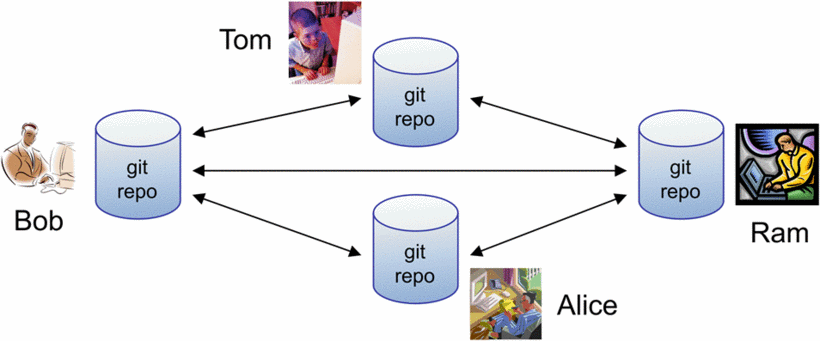
\includegraphics[width=1.0\textwidth]{decentralised_git.png}
\caption[Distributed revision-control with Git]{Distributed revision-control with Git. Figure taken from \cite{TorvaldsGit}.}
\label{decentralised_git}
\end{figure}
Git\cite{TorvaldsGit} is a modern code version-control system which uses distributed revision-control. The main difference with other version-control systems, say Subversion is, that Git is fully distributed. That is, a developer can make some changes on their own machine, and without accessing the main repository they can commit their changes to the local machine, as the local machine will have a valid Git repository. Later the developer can push changes from the local repository to any other machine which it has access to, as seen in the figure \ref{decentralised_git}. Usually there is a dedicated `origin` computer which holds the up to date version of a repository, and with which the developers are communicating. This approach makes it easier to develop software when internet connectivity is poor (as we can still work on a project locally), but introduces other issues, such as merge-conflicts. It was developed to help the Linux kernel developers with proper version control system. Since its development in 2005, it has been widely used by open-source projects as their primary VCS, such as the Django Project\footnote{https://www.djangoproject.com/}, Ruby on Rails\footnote{http://rubyonrails.org/} or jQuery\footnote{https://jquery.com/}.
\subsection{Git snapshots - how does the version control works}

Git stores data differently to other major VCSs. Rather than storing for each file the list of changes, git stores the whole repository at each revision point in the history. For efficiency if a file hasn't been changed at a commit, rather then storing the file again, Git only stores a pointer to the last identical file in the previous revision as in figure \ref{snapshot_git}. We can think of a Git repository as an ordered list of snapshots. To view differences (using the \texttt{git diff} command) Git looks up the differences in a repository between two snapshots. In this definition, version control is simply done by storing (committing) at various times the state of our repository, directory structure.
\begin{figure}[h]
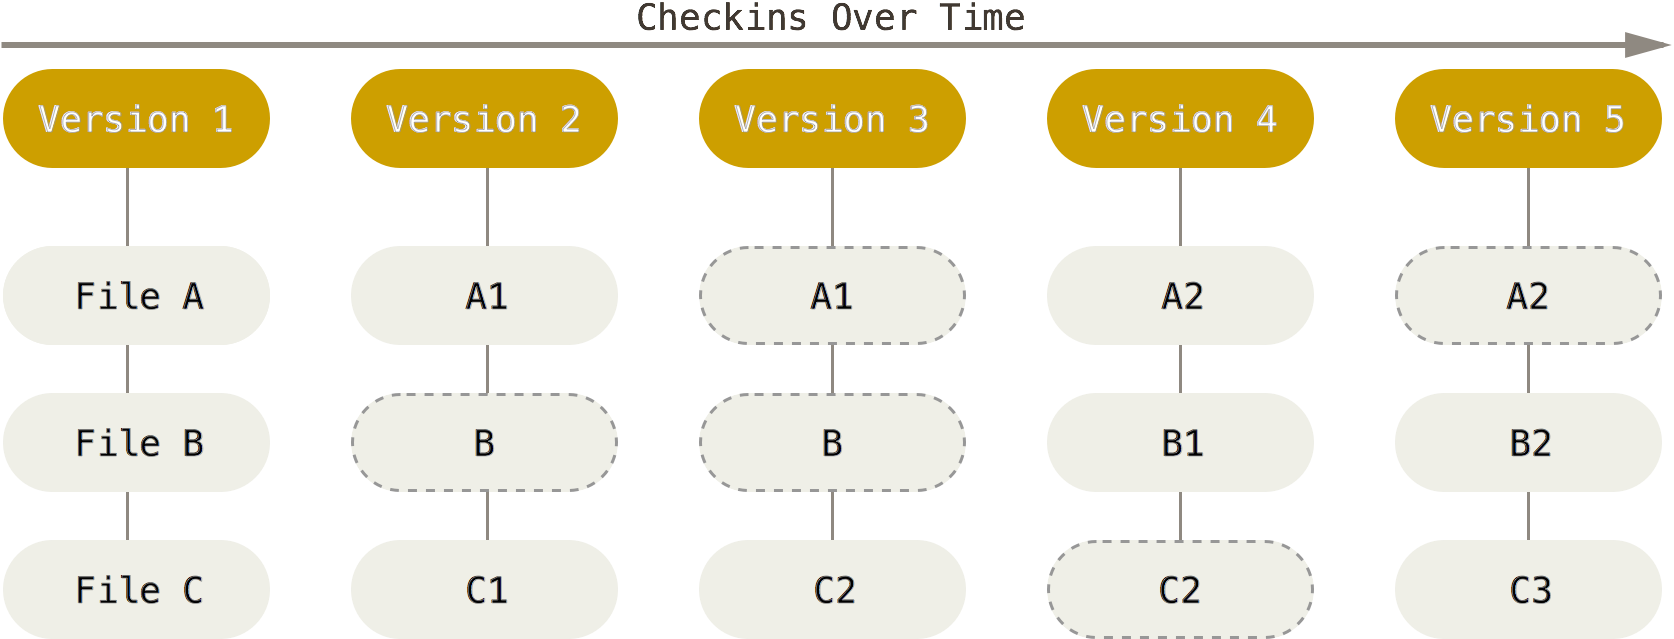
\includegraphics[width=0.8\textwidth]{snapshots_git.png}
\centering
\captionsetup{width=0.8\textwidth}

\caption[Snapshots in Git]{Snapshots in Git, pointers to files have striped lines. Figure taken from https://git-scm.com/book/}
\label{snapshot_git}
\end{figure}
\subsection{Git File structure}
At each revision point in a Git repository we can think of data as a small file structure. Objects in a Git snapshot can either be blobs or trees: Blobs correspond to files whereas trees correspond to directories and subdirectories under the repository's root directory. At each point in the history of a repository Git stores a commit object, which stores the meta-data about that commit, for example: the author, the time committed. Furthermore, this commit object has pointer to a tree object, corresponding to the root directory of the repository as seen in figure \ref{commit-and-tree_git}. Furthermore, each tree can have a pointer to many more trees or blobs. Blobs, as they correspond to files, do not have any children. Each commit has a pointer to it's parent(s), except the initial commit which doesn't have parent(s).
\begin{figure}[h]
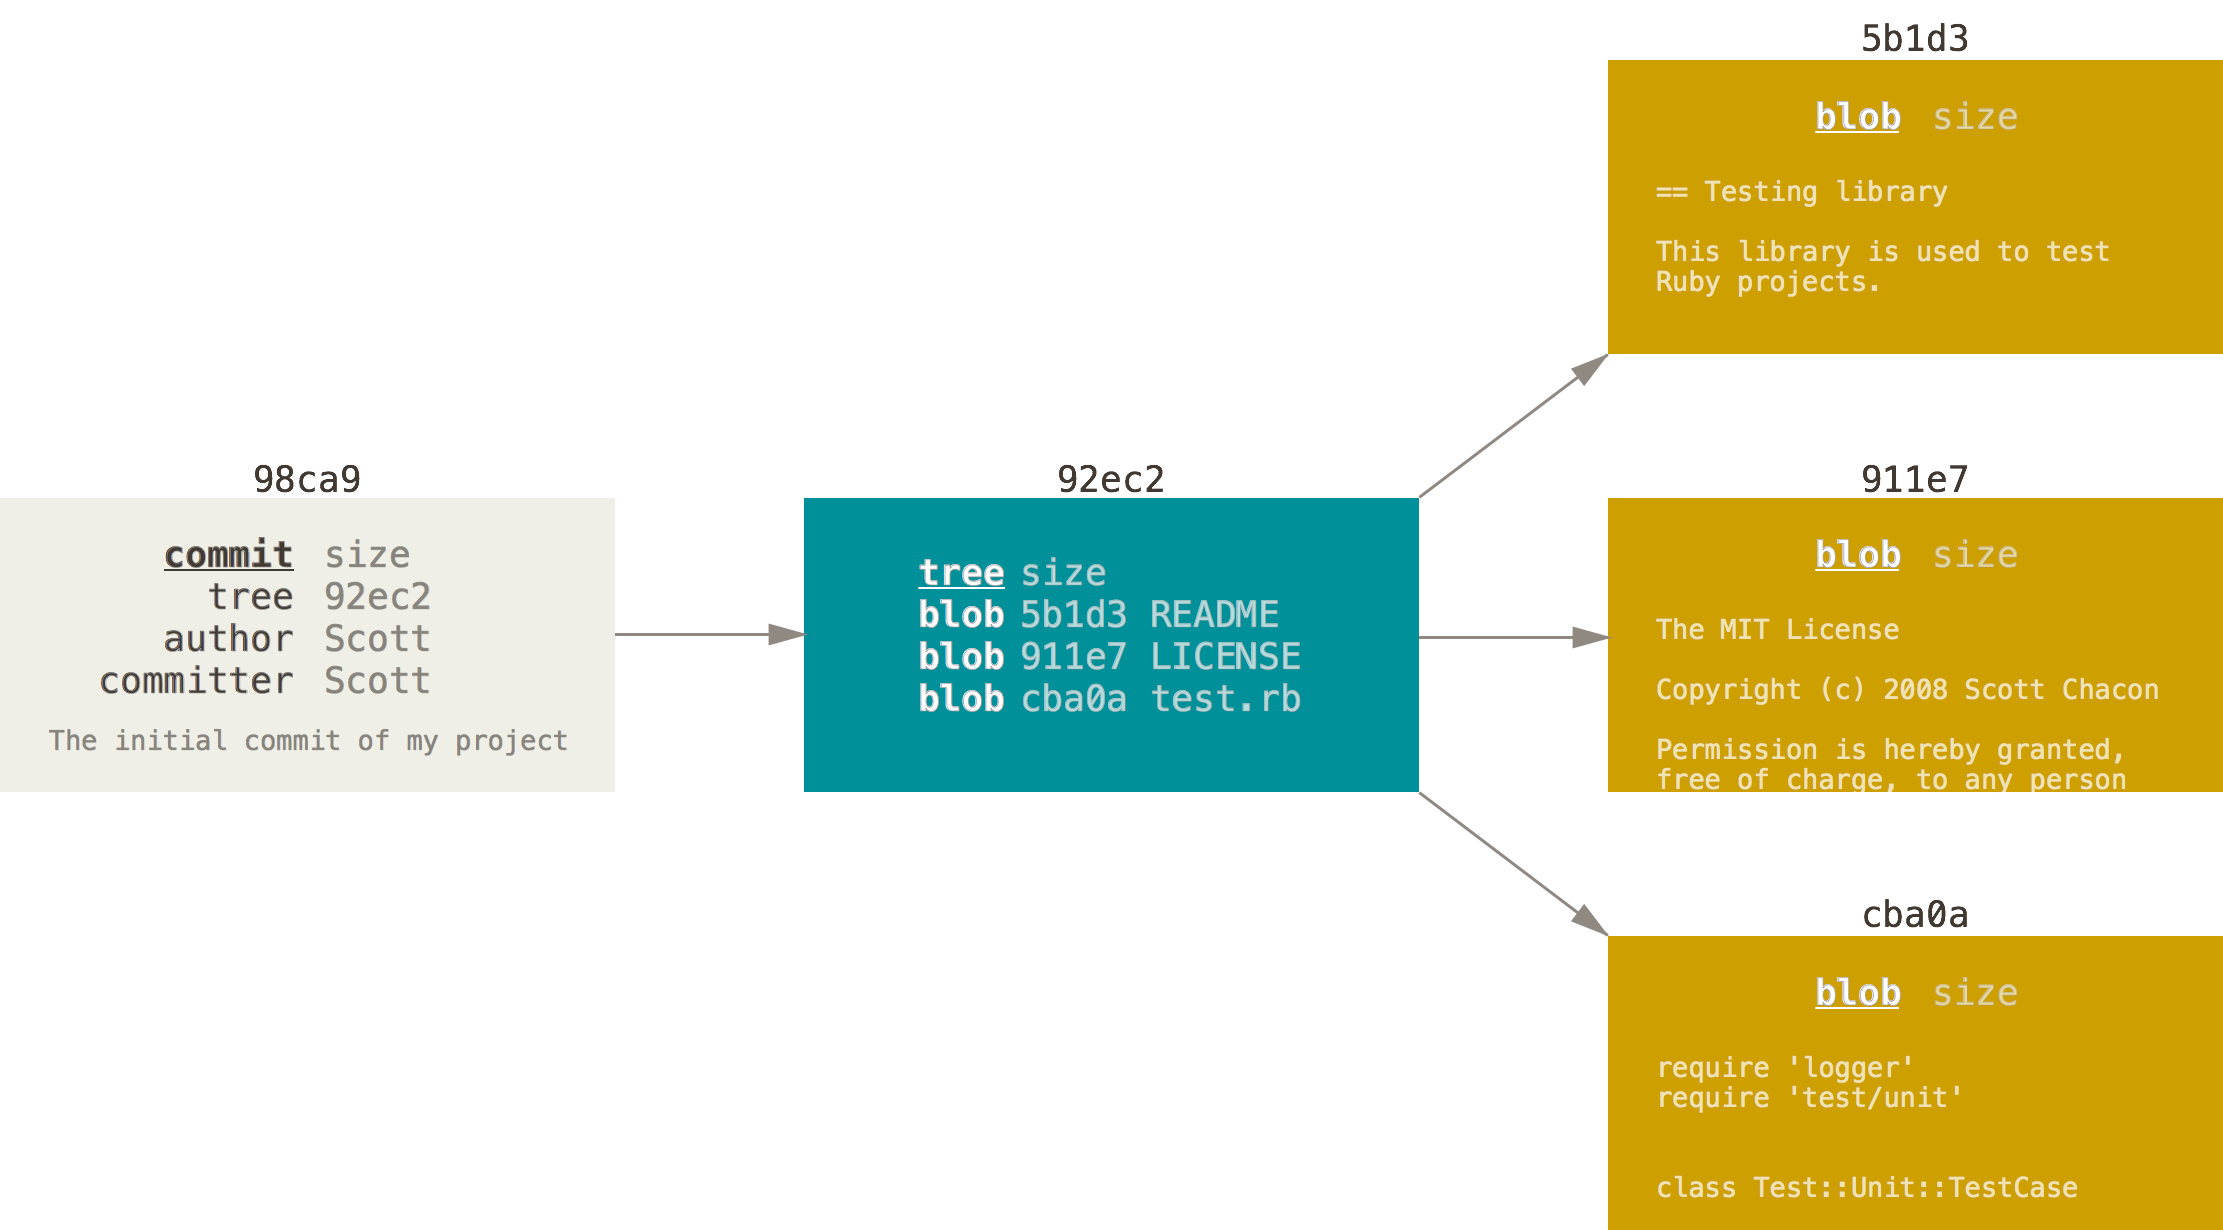
\includegraphics[width=0.8\textwidth]{commit-and-tree_git.png}
\centering
\caption{Git file-structure for a given commit}
\label{commit-and-tree_git}

\end{figure}
\subsection{Branches in Git}\label{gitbranches}
Branches are an important feature of Git, but they make mining repositories harder, as they introduce new problems to be tackled. They allow a non-linear development in a decentralised manner, meaning that developments can make their own changes locally, and later join/merge these changes together. 

As each commit is simply an object with some meta-data, which stores a pointer to a snapshot, a branch is simply a pointer to one of these commits. The branch named "master" is the default branch (although this can be changed), after initialising a repository you are given a "master" branch which will store a pointer to the latest commit made. When a new branch is created, Git creates a new pointer to the commit viewed at that moment. Git knows which branch is active at any time by storing a special pointer called "HEAD" which is a pointer to the active branch object.
\begin{figure}[ht!]
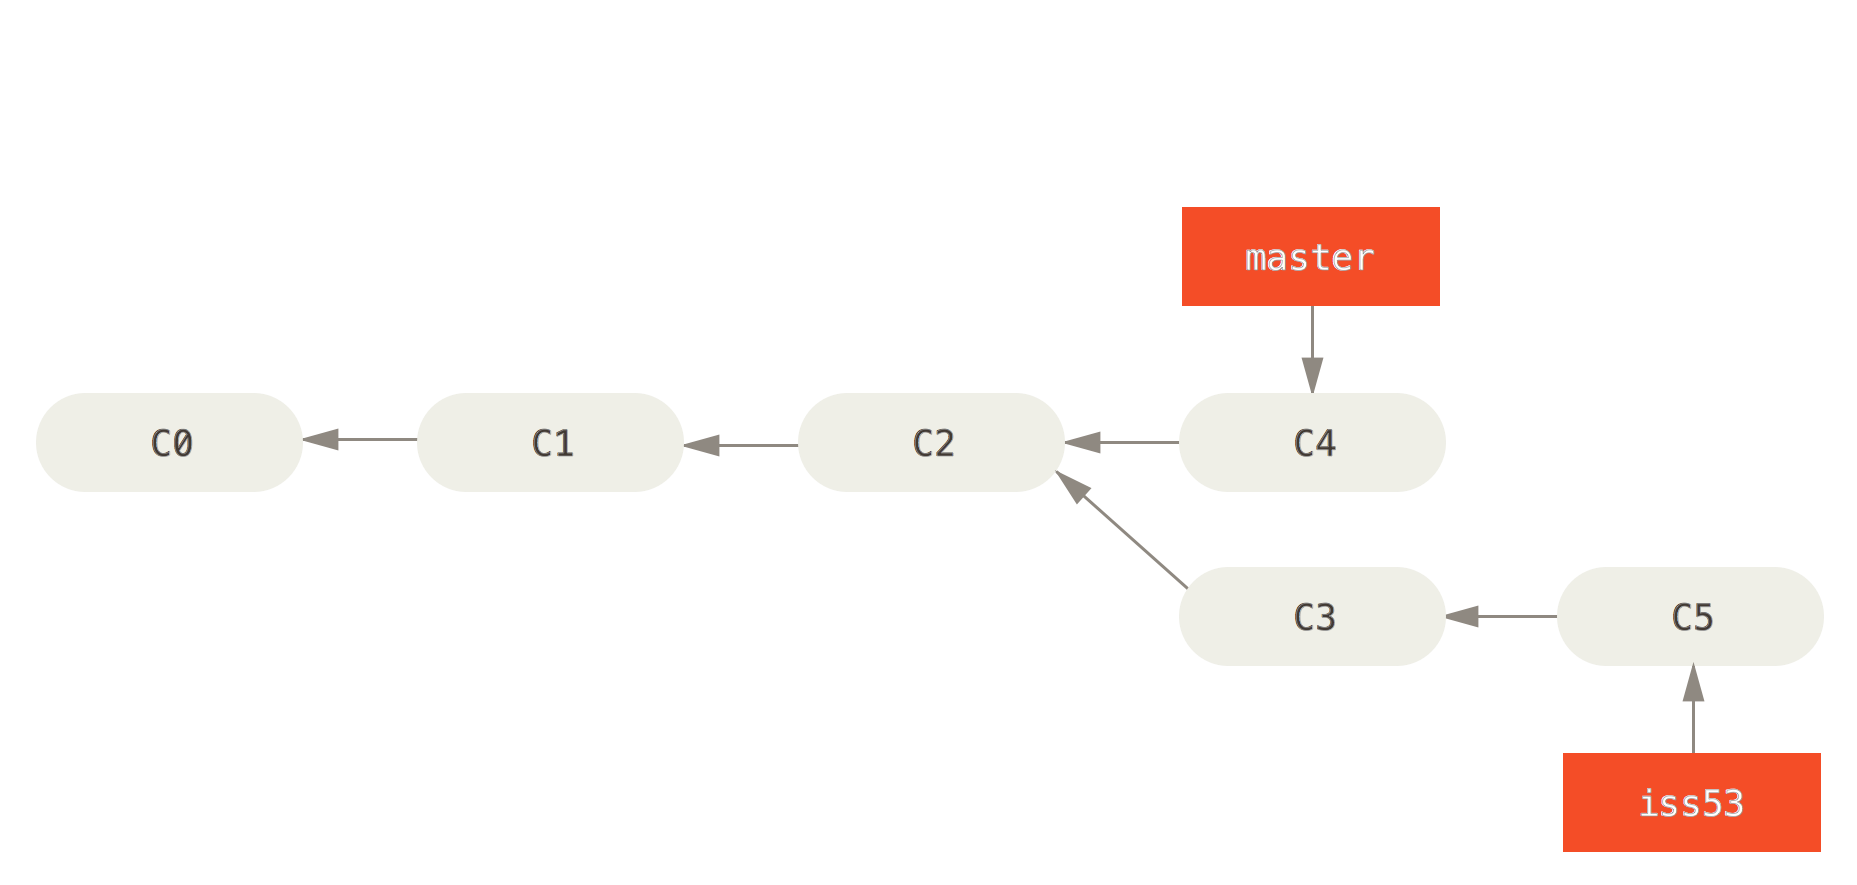
\includegraphics[width=0.8\textwidth]{basic-branching_git.png}
\centering

\captionsetup{width=0.8\textwidth}
\caption[Basic branching in Git]{Basic branching in git, with two branches: `master` and `iss53`.}
\label{basic-branching_git}
\end{figure}

It is possible to diverge two branches, as seen in figure \ref{basic-branching_git}. There starting from commit C2, some changes were made on branch `master` which resulted in commit C4. Then, from C2 also some changes were made on branch `iss53`, which resultsed in branches C3 and C5. We can see from the diagram that C4 and C3 have the same parent, C2.

Following this logic, you can also merge two branches, that is for example include the changes (that is the set of commits) made on branch B1 to the changes made on B2. If B1 and B2 are on the same linear path, we can simply fast forward, that is point the pointer of B1 to the same place when B2 is pointing. Otherwise, we need a real merge, which can be tricky to do automatically. There are two cases here:
\begin{enumerate}
\item There are no merge conflicts. This means that there is no single file which were changed/overwritten on both branches. In this case Git will handle merging automatically through a so-called "recursive-merging" algorithm.
\item There are merge conflicts. This means that there is at least file which has been modified by both branches B1 and B2. In this case Git will merge the files that it is able to merge, and for those where the conflict arose it will place some readable text to tell the user where the conflict is. The user will have to manually go to each file and resolve the conflict, and commit the new changes later. There exist automated tools for merge-conflict resolution, which automate the last two steps during the merging command itself.
\end{enumerate}

When a merge occurs Git will create an automated merge commit, which will contain the information about the which commits were merged together, that is this commit will have at least two parents. The changes contained by a merge commit are also visible on the branch they were really made, this is an important feature if you want to view the repository as a linear history of commits. 

As each commit can be a parent of one or more commits and similarly each commit can have zero ore commits we can treat the history of a repository as a Directed Acyclic Graph (DAG). This is a big difference between other VCS softwares as in non-distributed VCS branching is harder to achieve, and once we have it it is quite hard to backtrack which branches were used by which user and when[need better explanation+reference here]. The DAG representation comes handy when analysing different user activities, but it introduces several new problems, because when we are mining a repository we might want to check each path in a repository. 

It is also possible to view each branch as a linear set of commits (even when some branches were merged into this branch). Commits will appear in their order of committed time, regardless on which branch were they made. This linear representation will also contain all the merge commits, which will be the ones with at least two parents. This means, that when going through this history merged changes will be visible twice: once in their original commit (made on some branch B1) and once in the merge commit of branches B1 and B2 say.
\section{GitPython}

\subsection{Overview}
GitPython\footnote{https://github.com/gitpython-developers/GitPython} is a python package developed by Sebastian Thiel\footnote{https://github.com/Byron} as a purely python high-level tool for interacting with Git repositories. By using it, one is able to do everything via Python: create new repositories, commit changes, checkout branches etc. Each Git object has its own representation in GitPython, and each object is stored in a object database to achieve lower memory overhead. In fixcache, GitPython will only be used to access for the following tasks:
\begin{itemize}
\item Getting the list of commits (for the \texttt{master} branch) in chronological order
\item To determine differences in files between two commits
\item To keep track of each files history: number of changes, faults and lines at each commit.
\end{itemize}
\subsection{The object database}\label{dbbackend}

\begin{figure}[h]
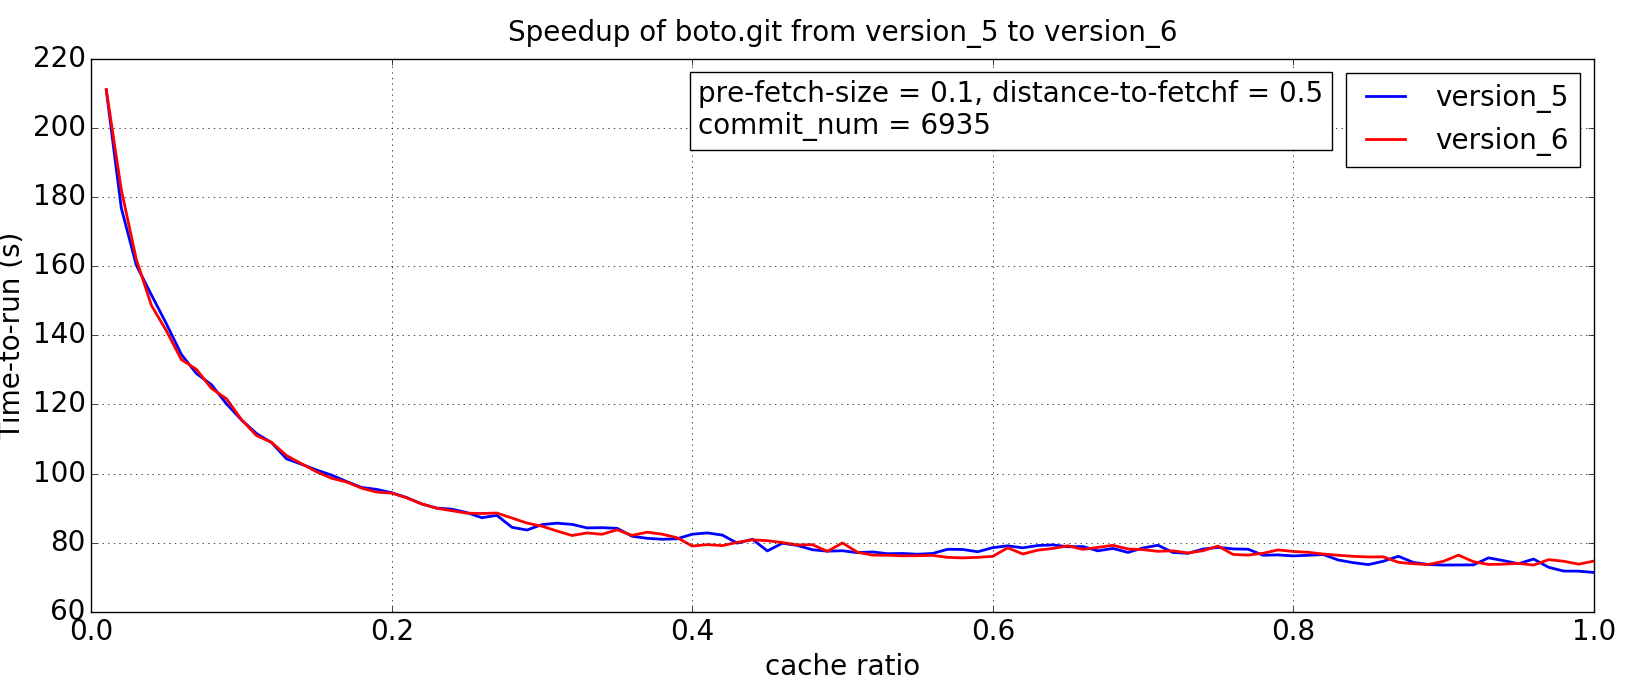
\includegraphics[width=1.0\textwidth]{db_backend-1.png}
\caption{Showing time-to-run of backends \texttt{GitDB} (version\_5) and \texttt{GitCmdObjectDB} (version\_6) for boto.git repository}
\label{boto_gitdb}
\end{figure}

Behind the scenes GitPython is using gitdb\footnote{https://github.com/gitpython-developers/gitdb} for accessing a git reposiotry. This is an efficient way of accessing data, as gitdb only operates on streams of data rather than the whole objects, so it actually requires small amount of memory. There are two options here, either we use the default \texttt{GitDB} (implemented by the gitdb package) or the \texttt{GitCmdObjectDB} which was only added to the GitPython. The first one, according to the Thiel \textit{"uses less memory when handling huge files, but will be 2 to 5 times slower when extracting large quantities
small of objects from densely packed repositories"} while second one \textit{"uses persistent git-cat-file instances to read repository information. These operate very fast under all conditions, but will consume additional memory for the process itself. When extracting large files, memory
usage will be much higher than the one of the \texttt{GitDB}"}.
\begin{figure}[h]
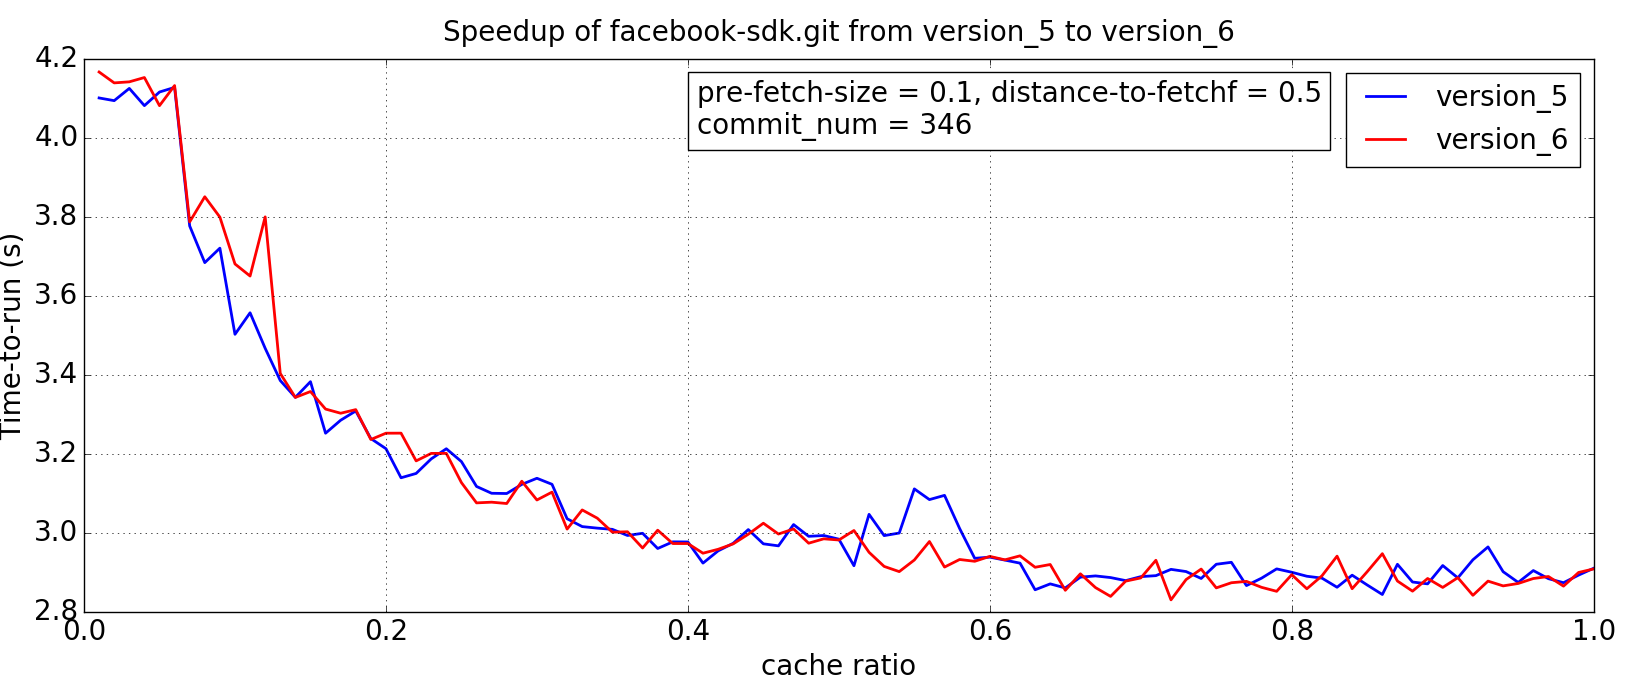
\includegraphics[width=1.0\textwidth]{db_backend-2.png}
\caption{Time-to-run of backends \texttt{GitDB} (version\_5) and \texttt{GitCmdObjectDB} (version\_6) for facebook-sdk.git repository.}
\label{facebook-sdk_gitdb}
\end{figure}

Figure \ref{facebook-sdk_gitdb} and \ref{boto_gitdb} show the time-to-run in seconds for both. As it can be seen, there is not a significant difference in the running time, so the default (\texttt{GitDB}) back-end was used for all further analyses.
\cleardoublepage
\chapter{Implementation}
This chapter summarizes the main components implemented to run \fxch{}. It first explores a very high level view of all modules, and then it describes all components in more detail, together with any implementation difficulties.
\section{Design overview}

The algorithm is implemented in Python using its 2.7.6 release. The implementation has several modules which handle different parts of the algorithm. The main module is the Repository which implements the algorithm itself. It uses several back-end modules, such as Parsing, File management and Cache. Figure \ref{fixcache_flowgraph} on the next page shows these main modules and how do these modules depend on each other.

\begin{figure}[h]
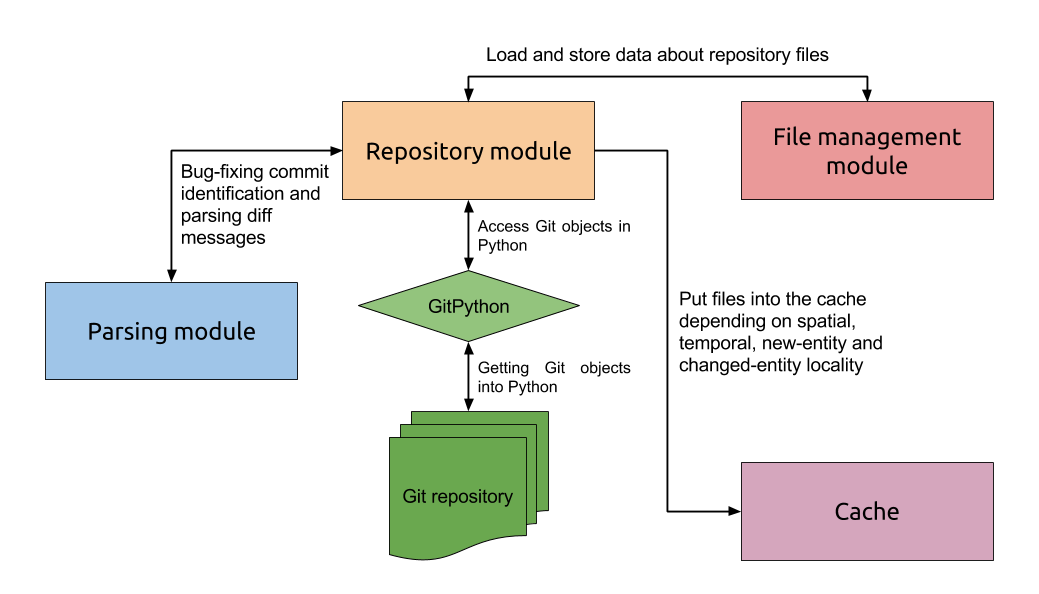
\includegraphics[width=1.0\textwidth]{fixcache_flowgraph.png}
\label{fixcache_flowgraph}
\caption{Core modules and the interaction between them.}
\end{figure} 

\paragraph{Parsing module}Accepts data from Repository (as can be seen on figure \ref{fixcache_flowgraph}, and then it processes that data and sends the parsing result back to the Repository. It is essentially a collection of functions which do different parsing used by \fxch{}: flagging important lines, parsing \texttt{git diff} messages to get the line numbers of deleted lines and flagging bug-fixing commits from the commit message.

\paragraph{File management module}Implements a layer for representing files, file-sets and distances between files. The classes implemented by this module are used both by the Cache module and by the Repository module, however only the latter accesses File management explicitly. We can think of this module as a database which can be queried by the Repository module for different types of data such as file-metrics and relationships between files.

\paragraph{Cache module}This module contains the \texttt{Cache} class which represents our cache when running \fxch{} in our \texttt{repository} module. Instances of this class will store how good the algorithm is, that is they will keep track of number of hits and number of misses. The Repository module will send new files to our Cache module, which will handle additions to cache, and removals if the cache is filled. The removals are handled implicitly, hence the one-way line in figure \ref{fixcache_flowgraph}.

\paragraph{Repository module}This is the main module which runs \fxch{} itself. It communicates with all the other modules (requesting existing files, adding new files, updating the cache, parsing data), and handles the communication of these module between themselves. Also it will read the the Git repository (through GitPython on which we are currently running \fxch{} itself. The communication of Repository with other modules differ by module. In the figure \ref{fixcache_flowgraph} the striped line means that there are no \texttt{File} or \texttt{FileDistance} (these are described later) instances involved. The continuous line on the other hand, means that we are sending and receiving these objects from other modules. For example, Repository will request \texttt{File} and \texttt{FileDistance} objects based on files' paths and File management will return the correct instances. Similarly, Repository will send new \texttt{File} instances for the Cache module to process, which will insert them into the cache itself.
\clearpage
\section{Back-end modules} Back-end modules are used by the Repository module, when running \fxch{}. They are the layer which handles the abstraction of objects and object metrics used by \fxch{}.
\subsection{Parsing module}\label{parsing}
The Parsing module parses data arriving from the Repository module, as it can be see in the figure \ref{parsing_module} representing the data-flow through the module. The three key functionalities implemented are: deciding whether a line is "important" or not; getting the numbers of deleted lines from the output of a \texttt{git diff} command; parsing the commit messages to identify fixing commits. 
\begin{figure}[h]
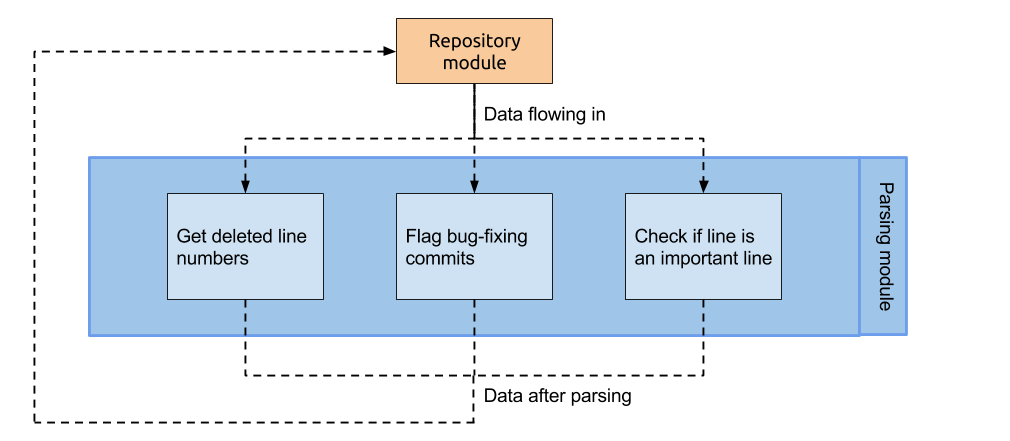
\includegraphics[width=1.0\textwidth]{parsing_module.png}
\caption{Data-flow through the Parsing module}

\label{parsing_module}
\end{figure}
\subsubsection*{Check if line is important}
When identifying bug-introducing commits, we are using the SZZ algorithm\cite{SZZ} (explained in section \ref{szz}), which has a step of finding which lines are contributing to the bug. This algorithm has been criticised by Kim et al.\cite{KimZim} as when identifying these lines, they are all treated equal. This will ultimately introduce plenty of false positive lines, that is lines which were changed during a bug-fix but had no contribution to the bug whatsoever.
\begin{figure}[h]
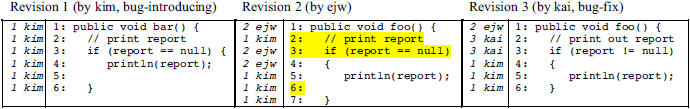
\includegraphics[width=1.0\textwidth]{automatic_identification.jpg}
\caption{Example of changes between revisions (3rd fix is a bug-fix change). Figure taken from \cite{KimZim}.}
\label{automatic_identification}
\end{figure}

For example if we look at the figure \ref{automatic_identification} we can see three revisions. When we look at the bug-fixing revision (Revision 3) we can see that it changed lines \#2 and \#3 and it removed line \#6.
SZZ would identify all of these lines as buggy lines, whereas we can see that truly only \#3 should be treated as a buggy line, because \#2 is a comment line and \#6 is blank line.
Several improvements have been proposed by Kim et al. to reduce the number of false positives\cite{KimZim}, out of these we are only checking if a line is blank/empty or if it is a comment line. As this implementation is for Python repositories, to identify comment lines we parse each line and identify whether it starts with \texttt{\#} (the comment symbol in python). Multi-line comments are ignored, as python uses the same syntax for them and for mutli-line strings. 

This important line checker merely outputs an approximation for the lines which are truly important (that is they contributed to the bug fixed), usually it will return a bigger set. Further approximating the true set would require more techniques mentioned by Kim et al., but getting the exact set is computationally impossible\cite{KimZim}. 
\subsubsection*{Getting deleted line numbers}
An essential part of the \fxch{} algorithm is identifying which lines were removed between two revisions. This information is later used when identifying the so-called "bug-introducing" commits with the SZZ algorithm.

Our module will accept the output of a \texttt{git diff} command for each file in the commit, and it will parser this output to get the line numbers which were deleted in that \texttt{git diff} (where the difference is what changed between the commit and it's parent commit), that is the line numbers of all the lines starting with "\texttt{-}" in our \texttt{git diff}.
\subsubsection*{Identifying bug-fixing commits}
For each commit the algorithm looks at, we need to decide whether it is a fixing-commit or not. To identify these commits, we need to parse the commit message itself. If the commit message is accepted by any of the below regular expressions (following Sadowski et al.\cite{Sadowski}), we flag it as a bug-fixing commit. 
\clearpage
Regular expressions used to parse commit messages:
\begin{itemize}
\item \texttt{r'defect(s)?'}
\item \texttt{r'patch(ing|es|ed)?'}
\item \texttt{r'bug(s|fix(es)?)?'}
\item \texttt{r'(re)?fix(es|ed|ing|age\textbackslash s?up(s)?)?'}
\item \texttt{r'debug(ged)?'}
\item \texttt{r'\textbackslash\#\textbackslash d+'}
\item \texttt{r'back\textbackslash s?out'}
\item \texttt{r'revert(ing|ed)?'}
\end{itemize}
\subsection{File management module}
When running \fxch{}{} we need to somehow store data about the files we looked at so far (their number of faults, changes, their LOC) and also we need to store the distance between any two files in our system, at any commit. A  good implementation would be able to tell for any two files $f_1$ and $f_2$ that what is their co-occurrence (which is reversely proportional to their distance) at any commit $n$. The figure \ref{filemanagement_module} below shows a high level view of the File management module, and how data-flow through this module works.
\begin{figure}[h]
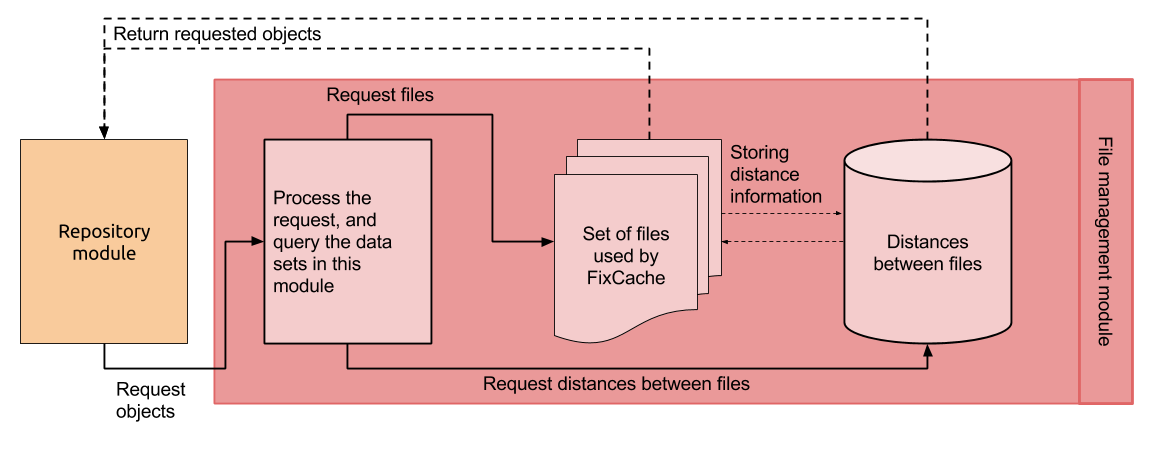
\includegraphics[width=1.0\textwidth]{filemanagement_module.png}
\caption{Data-flow through the File management module}
\label{filemanagement_module}
\end{figure}

As it can be seen from the figure, Repository requests objects (Files or Distances) from the File management module, and the module will return the requested objects from a set of files or from the distance database.
\subsubsection*{Processing requests}
When requesting files, the Repository module accesses them only by their file-path. That is, it queries every \texttt{filemanagement.File} object by it's file-path, and the File management module will either return the corresponding file, or if it did not exist before, it will create a new file with the queried path, and return the newly created file. We can think of this as a dictionary functionality implemented by File management, with an extension that if a key looked-up is missed, this module will create the corresponding value, rather than throwing a \texttt{KeyError}.

Similarly for file-distances, Repository will query by file-path, only this time the request will contain two paths (of the files we want to know the distance of). From these two paths, the Distance-database will create a key, and as before, it will return the corresponding value, or create a new \texttt{Filemanagement.Distance} object. The key-generation is fairly simple:
\begin{gather*}\label{distance_key} 
	\forall f_1, f_2\ files \\
	key(f_1, f_2) = \begin{cases}
						f_1.path+f_2.path &if\ f_1.path > f_2.path\\
						f_2.path+f_1.path &if\ f_1.path < f_2.path\\
						error &otherwise: two\ paths\ equal, f_1 == f_2
					\end{cases}
\end{gather*}
That is we will append the shortest path to the longest path for any two files. If the two paths are equal, it means that the two files looked at  are also equal, and we need to throw an error. Generally, this will never happen in this \fxch{} implementation, as we never query the distance with the same path.
\subsubsection*{Storing file information}
For each file in the repository looked at when running \fxch{} we create a \texttt{filemanagement.File} object indexed by it's path, which will store the basic information needed by \fxch{} as mentioned above. Whenever an file-related event occurs during our \fxch{} run we need to change or update the internal data of the file involved in the event so that it has a correct state when used by \fxch{}. There are three three major file-events:
\begin{itemize}
\item Changed file: whenever a file is committed, we need to record this change at that commit. First we added the commit number to the changed-commit-list (which stores all the commits at which the file was changed). Then we need to update the LOC for that file, where the amount of lines changed will be equal to $added\_lines - deleted\_lines$.
\item Fixed fault: at each bug-fixing commit $bfc$, for each file involved we mark that there was a fault associated with that file, and that this was fixed at $bfc$. This is later not used, as we are using LRU cache-replacement policy, but it could have been used with different cache-replacement policies which take the number of faults and their occurrence in time into account.
\item Reset the file: To complete an analysis we need to run \fxch{} 1500 times (for the cache-ratio analysis). If our repository, say has a 1000 files, we would create 1.5 million \texttt{filemanagement.Files}. This would be rather inefficient, so instead we reset all the objects present in our File-set and Distance-database: we set their internal parameters to their initial values.
\end{itemize}

When updating these objects after an event occurred we do not request every file, and do the update one-by-one. Rather, the output of a \texttt{git diff --stat} command is passed as data to the File management module, which will update and return files accordingly. In Git, this output looks like the following:

\begin{lstlisting}
setup.py | 11 ++++++++++-
 1 file changed, 10 insertions(+), 1 deletion(-)
\end{lstlisting}
Luckily we do not need to parse this, as GitPython already has a parser, which will parse it and create a nested Python dictionary. For the output above, this dictionary will look like this:
\begin{lstlisting}[language=Python]
{ 
	u'setup.py': {
    	'deletions': 1,
	 	'lines': 11,
	 	'insertions': 10
	}
}
\end{lstlisting}
Each changed file's path will be a key in this dictionary, and the corresponding value will be an another dictionary with three keys: \texttt{deletions, lines, insertions}. 

Our module will use this parsed \texttt{diff} data to update the files (changes, faults and LOC) in our File-set.: if they already existed update, if they did not create a new \texttt{File} instance. Furthermore we clean-up deleted files: we assume that each file is deleted when their LOC (lines-of-code) becomes zero.

After updating the data for each file and creating new files, it will return a list of tuples, where the second value of a tuple will be the actual \texttt{File} instance, and the first value will be either \texttt{'changed'} or \texttt{'deleted'} or \texttt{'created'} dependant on what happened to that file between the \texttt{diff}-ed commits we are viewing.
\subsubsection*{Distance-database}
In order to implement the temporal-locality used by \fxch{} we need to know the co-occurrence of any two files at any commit. To do that, for each two files committed together a \texttt{filemanagement.Distance} instance will be created and stored in the Distance-database. This instance will have a list of commit numbers representing the commits when the two files were changed together. That is, for each two files in a commit, we either update the corresponding \texttt{Distance} object, or we create a new one if it has not yet existed.

The Repository module queries these \texttt{Distance} objects by a key generated from the two file paths of which the distance we are looking for (as explained in \ref{distance_key}). Again, when a request is sent, either we return a already existing object, or we create a new one and return that. Whenever two files are committed together, the Repository module will query the Distance-database to get the \texttt{Distance} object, and it will update the co-occurrence for that object.

The Distance-database is also important when determining which files are the closest ones to a given file $f$ at a given commit $c$. In this case, the Repository queries the Distance-database with one file path ($f.path$ in this case), and asking for $k$ closest, files, and the database will respond with a list of \texttt{File} objects (at most $k$ number) which have the higher co-occurrence with the queried file.
\subsection{Cache implementation}
\fxch{} uses the notion of a file cache, which has some limited number of files in it. We can think of it as a bucket, where we can put some files in, and when the bucked is filled, it will automatically take care of cleaning up some other files in order to make space for new arrivals. The \texttt{cache.Cache} class is responsible for keeping track of files which are in the cache, counting hits, counting misses and removing files (according to or LRU policy). The figure \ref{cache_module} shows the cache handles the addition of new files.

\paragraph{Preprocessing}
Before putting the files into the cache, there is a pre-processing step, which will check if either of the files is already in our cache. If so, we will simply discard those files to avoid duplicates. This step is important as our cache needs to know exactly how much free space is required upon new arrivals.

The preprocessing step may also include sorting, if the cache is smaller than the number of files we want to insert. In this case, we need to sort them so that later they obey the LRU cache-replacement policy.
\begin{figure}[h]
\centering
    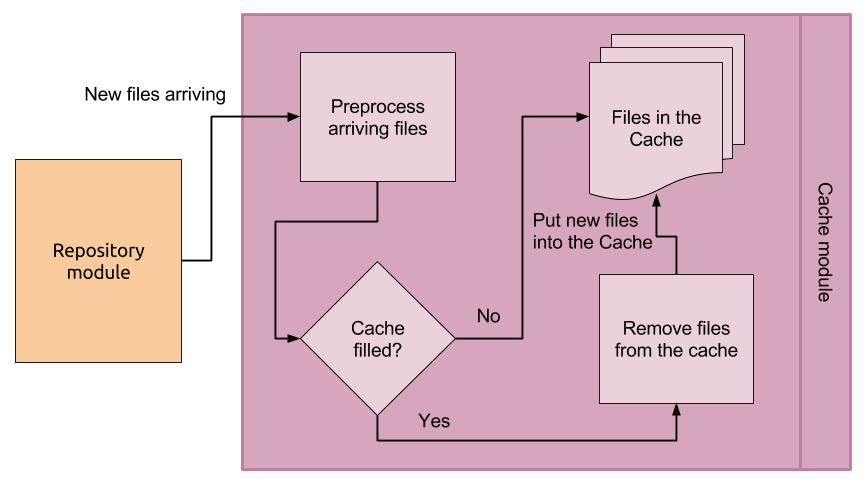
\includegraphics[width=0.75\textwidth]{cache_module.png}
  \caption{Adding new files to the Cache and processing them.}
  \label{cache_module}
\end{figure}

\paragraph{Adding new files} After preprocessing we can add the arriving files to our cache. We first look-up how much space do we need, and remove files accordingly. Once the required space has been freed, we can safely add the new arrivals.

\paragraph{Removing files} We are not removing any files explicitly. The implementation itself will take care of clean-up, so that it will only discard files when our cache needs more space. As we are using the LRU cache-replacement policy, if we need a space of $k$ files, this module will select the top $k$ least recently used files and remove them from the cache.

\paragraph{Limiting the number of files}
Internally, files are stored in Python \texttt{set()} object, which does not allow duplicates, but it does not have a size limit by default. To actually have a limit in our cache implementation, all addition methods first look up how many files are currently in the cache, and subtract that value from the cache size to get how big is the currently available space. Removing files works accordingly to this: if we need more space, we remove as many files as necessary to get it.
\section{The Repository module}
This module is the central element of the \fxch{} implementation. It is connecting all modules together, and uses them to run and analyse the algorithm for different repositories. A \texttt{repository.Repository} class is instantiated for each Git repository we want to run \fxch{} on. Also, this module has two more classes, used only for evaluation purposes. 
\subsection{Implementing the SZZ algorithm}
The SZZ algorithm in this implementation is implemented inside the \texttt{repository.Repository} class, rather than a standalone module, as it is a core part of \fxch{}. The two functions which are implementing it are:
\begin{itemize}
\item \texttt{\_get\_diff\_deleted\_lines(self, commit1, commit2)}

Returns the deleted line-numbers (per file) between any two commits. Used to get the deleted lines between a commit and it's parent.
\item \texttt{\_get\_line\_introducing\_commits(self, line\_list, file\_path, commit)}

Once we have the line numbers which were deleted between two commits (commit and it's parent) we can for each file get the list of bug-introducing commits. This method uses the \texttt{git blame} (which, in GitPython outputs a nested list, where the first value of a list is a commit object, and the second value is a list of lines last changed - introduced - by that commit), and produces a list of bug-introducing commits.
\end{itemize}
The SZZ algorithm is used for identifying commits which introduced a bug, that is it is only called for bug-fixing commits. That is for each fixing change, we want to identify the starting points of a bug fixed by that change.
\subsection{Cache size initialisation} A key variable used by our algorithm is the cache-size. Upon each initialisation (or after reset) we need to set the cache-size which will be stay static throughout a single run of the algorithm. To calculate the cache-size, we need to set a variable called cache-ratio (a number between between 0.0 and 1.0), and from this we will calculate the cache-size the following way: we take the number of files in the repository at the last commit, and we multiply this number by the cache-ratio. We then take the floor of this number (if the floor is zero, we add one, as the cache-size cannot be zero). That is:
\begin{align*}
	cr = file\_count\_at\_last\_commit*cache\_ratio\\
	cache\_size = \begin{cases}
						1 & if\ floor(cr) = 0\\
						floor(cr) & otherwise
					\end{cases}\\
	where\ cache\_ratio \in (0.0\dots 1.0]
\end{align*}
To calculate the variable file-count-at-last-commit we need to traverse the Git tree at the last revision, and count the number of 'blobs' (objects representing files) in the tree. A strong assumption is made here, namely that the repository will always increase as history moves forward. 

\subsection{Setting variables} Once we calculated and set cache-size we can calculate other variables, such as distance-to-fetch (block-size) and pre-fetch-size as discussed in \ref{variables}. In the original paper all these variables are given as a percentage of file-count-at-last-commit, that is if file-count-at-last-commit = 100, then distance-to-fetch = 5\% means that we will fetch 5 files each time we use our spacial-locality.

Rather than using percentages, this implementation for both distance-to-fetch and pre-fetch-size uses between 0.0 and 1.0. Also, they are not ratios of file-count-at-last-commit, but rather of cache-size. That is if file-count-at-last-commit = 100, cache-ratio = 0.1 and distance-to-fetch = 0.5 then we will fetch $100*0.1*0.5 = 5$ number of files.

\subsection{Initialising commits} In Git each commit's identifier is a 40-digit long hexadecimal number generated by SHA-1 from the commit data, it is impossible to know just from the hash value what is the order of commits. Our \fxch{} is using integers as commit identifiers (the bigger the commit number, the later it happened), so a dictionary needs to initialised prior to running our algorithm. We first iterate through the list of commits (which is provided by GitPython) and at each commit we store the hash value of that commit as key, and it's order in the list as the value. Each time we want to access the order of any commit object, we can lookup this dictionary.
\clearpage
\subsection{Running \fxch{}}
\begin{wrapfigure}{r}{0.5\textwidth}
\begin{center}
\vspace*{-0.5in}
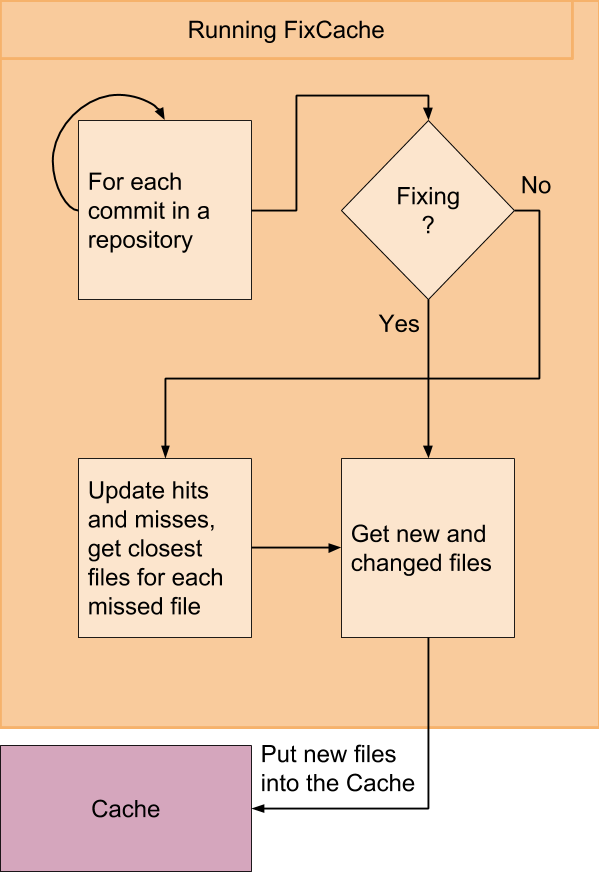
\includegraphics[width=0.48\textwidth]{repository_module.png}
\end{center}
\caption{Control-flow of \fxch{} inside the Repository module.}
\label{run_fxch}
\end{wrapfigure}
To run \fxch{} we need to call \texttt{run\_fixcache} on a \texttt{repository.Repository} instance; calling this method will run \fxch{} with the parameters currently set to some value. However, before running the algorithm itself, we need to find the repository for which we want to run it on. The Repository module will accept a string as an input, which will be the name of the repository we want to look at. The module will look for a repository with this name (under a pre-defined directory for repositories) and it will connect to it with GitPython, or throw an error if the repository is not found. Once we have connected to the desired repository we can run \fxch{}. The figure \ref{run_fxch} shows how the control-flow inside the Repository module works for a single run.

Between any two runs, we do not create a new connection with the repository, but rather we call a \texttt{reset()} function, which will implicitly reset the data found in all the other modules discussed earlier. This reset propagation will save memory, and also save some time as it is not necessary to redo the initialization step before each run.

Given all other modules, implementing \fxch{} is quite straightforward. Following the figure \ref{run_fxch}, a more detailed pseudo code would look like the algorithm presented on the next page.
\clearpage
\begin{algorithm}[H]
\KwData{A Git repository; Initial settings}
\KwResult{A cache with files projected to have bugs in the future}
\For{each commit in the commit list}{
	\uIf{commit has no parents}{Pre-load the cache with some initial files, starting with ones with the highest LOC}
	\uElseIf{commit has one parent}{
		\uIf{commit is a bug-fixing commit}{
			\For{each file included in this commit}{
				\eIf{file is in the cache}{
					Increase the number of hits
				}{
					Increase the number of misses and add file to the cache\\
					Find when the bug-introducing changes for this file, and put the closest-files at those commits to the cache					
				}
			}
		}
		
		Add some part of changed and created files at this commit to the cache.
	}
	\Else{This commit is a merging commit, so it may be disregarded.}
}
\caption{Pseudo-code for \fxch{}.}
\label{fxch_psd}
\end{algorithm}
\vspace{1em}
Cache additions are handled by our Cache module, while other operations (such as functions implementing SZZ) are handled by internal functions of \texttt{repository.Repository}.

In the above pseudo-code we have two if-statements: firstly how many parents does a commit have. If it has zero, it means that we are viewing the initial commit, so we need to pre-load the cache with some initial files (files with the biggest LOC). If it has one parent we proceed normally. If it has two or more parents it means that we have reached a merging commit, which we can disregard as the changes listed there already have been listed somewhere earlier in our commit history, as discussed in \ref{gitbranches}.

The second if-statement is when we are going through all files in our commit. If the file $f$ was already present in the cache, we increase the hit-count. Otherwise, we increase the miss-count and and this file to the cache (temporal-locality). Furthermore, we identify the commits which introduced (lets say: $bci_1, bci_2 \dots bci_n$ the bug-fixed in this commit, and add the closest files to $f$ at $bci_1, bci_2 \dots bci_n$ (spatial-locality).

Furthermore, for each commit we add the changed and updated files to the cache (new-entity and changed-entity locality). All these additions are bounded by some numbers specified by the pre-fetch-size and distance-to-fetch however these are omitted from the pseudo-code.
\section{Versions and errors}
There are several versions implemented: from version\_1 to version\_6, which differ in various aspects. Versions 1 to 4 are incorrect, these were the part of the development process, in which different bugs were discovered in different places, to list just a few:
\begin{itemize}
\item Negative indexing in python... Rather than throwing an error, Python allows negative indexing, which was an issue as the initial line-difference-counter was broken, and it was accessing negative line numbers in a file (which is a list of lines in Python). Everything worked, but it was functionally incorrect.
\item Broken diff-message parser. The output of a \texttt{git diff} command should be quite easy to parse, but the first implementation only looked for the first \texttt{@@} characters (which mark a meta-data line in the diff output), while several such characters might exist.
\item Localities were broken at the beginning. Rather than getting the files with biggest LOC the algorithm was getting the ones with smallest LOC. Similarly with last-recently-used vs. least-recently-used.
\end{itemize}
Version 5 and 6 only differ in that they use different object-database, as explained in \ref{dbbackend}, and version 5 is slightly faster.

As these versions are mostly only functionally incorrect, it still makes sense to compare them in terms of how fast they are relative to each other, as they have roughly the same number of computations. As it can be seen in the figure on page \pageref{fig:speedup} there is a massive speed-up between version\_1 and version\_5.
\section{Implementation difficulties}
\subsection{Using GitPython}
When using 3rd party software it is always key if the software we are using have a good or bad documentation (if it has a documentation at all). I have found that GitPython has generally good documentation, although some pieces (object reference, internal methods and variables of classes) lack proper definitions and clear type descriptions. There were times when the only way of finding out something about a certain class was to dive deep into the source-code of GitPython and try to figure out how is the certain class implementing functionalities provided by Git itself. This resulted in a slow implementation speed at the beginning of this project.
\subsection{Bottleneck: sorting}
During one run of \fxch{} there are several times when we have to select the "top objects from a set of objects". The "top objects" might mean "files with biggest LOC" or "least recently used files" or "closest files to a file at a commit". Usually the order does not matter after selection, we do not care whether the $k$ number of files are sorted after selection, as long as all selected files are "bigger" (ie. "have greater LOC" or "were used least recently" or "are closer than") than any file which was not selected. Also, for each of these selections the $k$ does not change throughout a single run of \fxch{}, as usually it's value is pre-calculated during initialization of the algorithm. On the other hand, $n$ changes from commit to commit.
\paragraph{Initial implementation}
Initially all these selection procedures were implemented by: first sorting the whole set of $n$ files, and then selecting the top $k$ elements. This is rather inefficient in two cases:
\begin{enumerate}
\item If $k << n$, then we are wasting time on an $\mathcal{O}(n\log(n)$ operation, while we could do in $\mathcal{O}(n\log(k))$ (using a selection algorithm explained on page \pageref{gettopk}, which for large n is clearly more efficient than sorting.
\item If $k >= n$, then we could just return the whole set of $n$ files, which is $\mathcal{O}(1)$ as the order after selection does not matter, thus we are wasting time again on sorting ($\mathcal{O}(n\log(n)$) instead of doing a constant-time operation.
\end{enumerate}
From the two possibilities above we can see that if $k$ approaches $n$ from above, we can not really improve on the algorithm itself.
\section{Speed-up}\label{gettopk}
\subsection{Alternative for sorting}
To achieve speed-up we need to implement a "select top k elements from n objects", mentioned in the previous section. This can be done Using a binary-min-heap, the pseudo-code looks like this:
\vspace{1em}
\begin{algorithm}[H]
\KwData{A list of $n$ sortable objects and $k$ an integer.}
\KwResult{A list of $k$ top objects from the list of $n$.}
heap = BinaryHeap()\\
\eIf{if $k$ is bigger or equal to $n$}{
	return the input list of objects.
}{
	\For{item in the object list}{
		\uIf{heap has less elements then k}{
			push the item onto the heap
		}
		\uElseIf{heap has k elements}{
			\uIf{item bigger smaller than heap.min()}{
				pop the smallest object from the heap, and push item onto the heap
			}
		}
	}
	return all the objects in the heap as a list.
}
\caption{Return the top $k$ elements from a list of $n$ sortable objects}
\end{algorithm}
\vspace{1em}
We need to have a binary min-heap, to keep track of what is the minimal item in the currently selected $k$ objects. If we find anything that is bigger than the current minimum, we either simply push that onto the heap, or if there is no space in the heap (that is the heap has $k$ elements) we pop the smallest item, and then insert the new one. The time complexity of insertion and pop operations for a heap of size $k$ is $\mathcal{O}(\log{k})$, and since we need to traverse all the objects, the above function has a time complexity bounded by $\mathcal{O}(n\log{k})$ as required.
\begin{figure}[h]
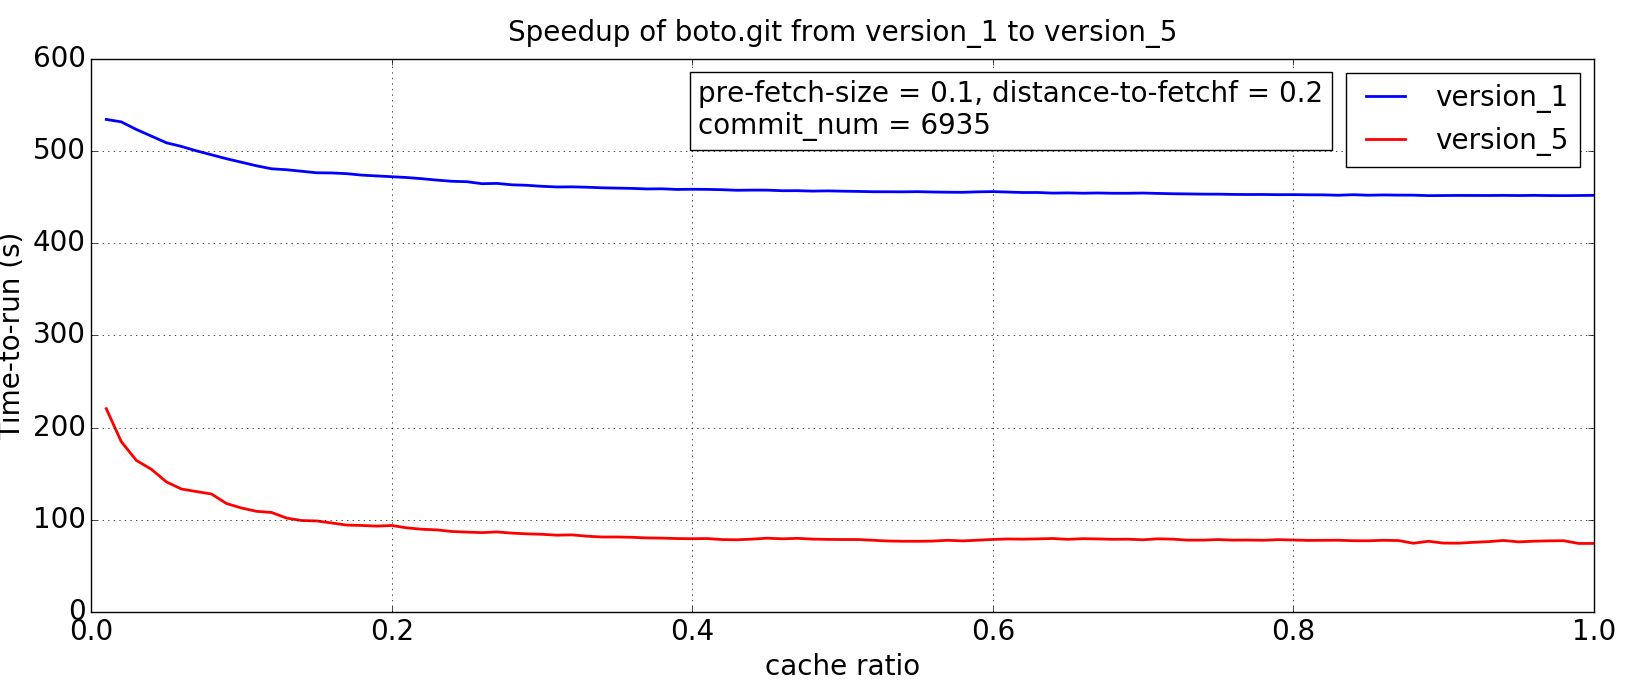
\includegraphics[width=1.0\textwidth]{speedup.png}

\caption{Speedup of boto.git and boto3.git between version\_1 and version\_5 with different cache-ratios}
\label{fig:speedup}
\end{figure}

We can see on figure \ref{fig:speedup} on the next page, how good is fast did it take for \fxch{} to run for a given cache-ratio. The figure is showing two versions: version\_1 (with sorting) and version\_5 (with "select top $k$ from $n$), and its clear that version\_5 is faster.
This speed-up is caused mainly by replacing sorting, as we will be using more linear operations (if $k >= n$) and $\mathcal{O}(n\log{k})$ operations, where for a single run $k$ is fix, and $n$ is changing.
A reason for this speedup is that whenever we increase the cache-ratio we also increase the cache-size, and the bigger the cache size, the bigger the pre-fetch-size and distance-to-fetch, so we will fetch more files, hence our "get top k elemens from n objects" algorithm explained in \ref{gettopk} will run in $\mathcal{O}(1)$ time more often, as $k$ (the number of files we are fetching) will increase with $n$ unchanged.
\subsection{Git diff with and without the --stat flag}
The command git diff outputs the difference between two snapshots (commits for instance). Without any flags/options set it will output the line-by-line difference with some metadata at the beginning for each file. If the task is only to get the basic information of how files changed it is good to use the --stat flag. With this Git will only outputs which file has had lines deleted and/or added, and how many lines this was. This second is more efficient in the background, due to how diff is implemented (reference here??).
\chapter{Evaluation}
\section{Repositories analysed and evaluated}
The algorithm was evaluated and analysed using five repositories: facebook-sdk.git\footnote{https://github.com/mobolic/facebook-sdk}, raspberryio.git\footnote{https://github.com/python/raspberryio}, boto3.git\footnote{https://github.com/boto/boto3}, boto.git\footnote{https://github.com/boto/boto} and django.git\footnote{https://github.com/django/django}. All these repositories were cloned, and \fxch{} was run on the locally: facebook-sdk.git was mainly used for testing purposes; raspberryio.git, boto3.git and boto.git was analysed completely; boto.git and django.git were used for evaluation. The repositories were chosen to have different number of commits, and to be mostly pure Python (except raspberryio.git which is only 43\% Python), also they have been used in earlier projects I was involved in, hence the idea to analyse them.

As all the repositories were cloned, the data presented here (such as the number of commits for a repository) resembles the data for the date when the repository was cloned, that is: 11-10-2015 for facebook-sdk.git; 22-04-2014 for raspberryio.git; 12-01-2016 for boto3.git; 18-01-2016 for boto.git; 28-03-2016 for django.git.
\section{Evaluation modules}
\subsection{Analysing \fxch{}}
To analyse and evaluate \fxch{} we need to run it several times each time with different parameters. The Analysis module contains different functions to perform different types of analysis. Out of the three key variables (cache-ratio, distance-to-fetch and pre-fetch-size) we fix one or two, and later we display the results found. The different analysis types implemented are listed below.
\subsubsection{\texttt{analyse\_by\_cache\_ratio}}Here, at a single analysis we fix both pre-fetch-size and distance-to-fetch, and run \fxch{} for 100 different cache sizes, that is cache-ratio $\in \{0.01, 0.02, 0.03 \dots 0.99, 1.00\}$ We run this for different pre-fetch-size and distance-to-fetch values, namely pre-fetch-size $\in \{0.1, 0.15, 0.2\}$ and distance-to-fetch $\in \{0.1, 0.2, 0.3, 0.4, 0.5\}$ That is, a complete analysis of this type will require $100*5*3=1500$ runs of \fxch{}.
\subsubsection{\texttt{analyse\_by\_fixed\_cache\_ratio}} 
Following the previous examples, here we fix the cache-ratio, and are interested in the best possible pre-fetch-size and distance-to-fetch for a given cache-ratio. We look at different cache-ratios, to be specific: $cache\_ratio \in \{0.05, 0.1, \dots 0.5\}$. 
\subsection{Displaying results}
We store all the results, for each analysis in .csv files. Once the .csv files were created, we read them and display the data using the matplotlib\footnote{http://matplotlib.org/} Python library. The Graph module is responsible for reading, and displaying the .csv files created by our Analysis module, as .png images using matplotlib.
\section{Evaluation over hit-rate}
\subsection{Results}
In the original paper \fxch{} is evaluated and analysed against the hit-rate, that is the ratio of cache hits over all cache lookups. It was found for several projects (such as Apache1.3, PostgreSQL, Mozilla and others in \cite{FixCache}) that the hit rate is between 0.65 and 0.95 for cache-rate of 0.1, pre-fetch-size of 0.1 and distance-to-fetch of 0.5.

For the same variables, similar results were found: hit-rate was always between 0.6 and 0.83. Also, for repositories with higher number of commits we usually had a bigger hit-rate, as we can see on the diagram on page \pageref{fig:v5_repos}. At cache-size = 0.2, we get an even better result of hit-rate which will be between 0.75 and 0.9. It seems that for bigger repositories (such as boto.git) the curve is smoother than for smaller ones, as one might expect.
\begin{figure}[th!]
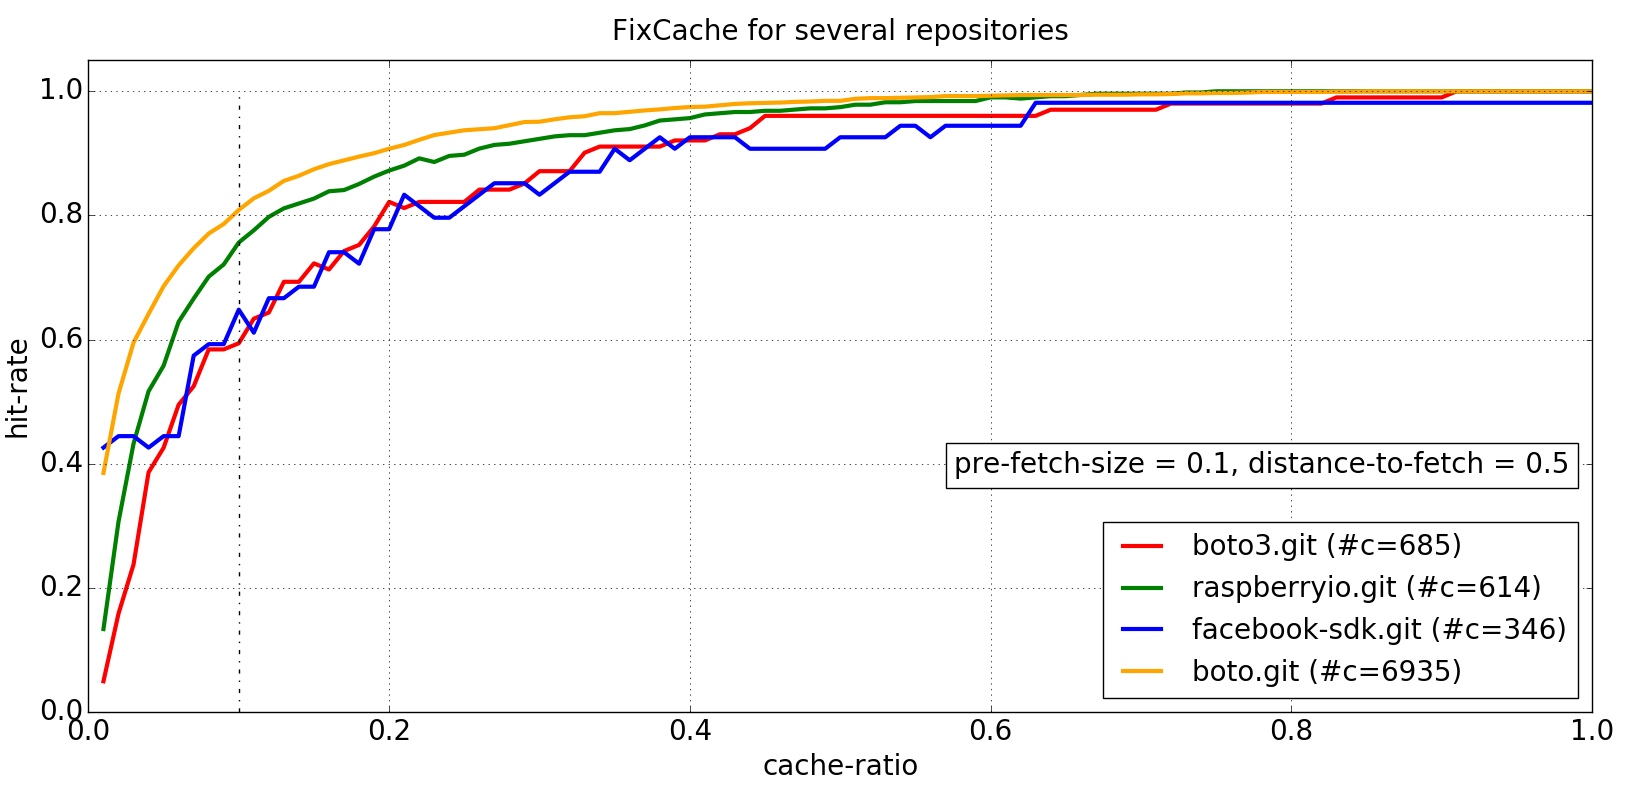
\includegraphics[width=1.0\textwidth]{plot_several.png}
\caption{Evaluation of \fxch{} according to hit-rate for different repositories}
\label{fig:v5_repos}
\end{figure}
\paragraph{What is the best cache size?}
From the figure \ref{fig:v5_repos} it can be deduced that the best hit-rate occurs around 0.2 of cache-ratio. For this ratio, for all possible distance-to-fetch and pre-fetch-size values the raspberryio.git has a hit-rate between 0.86 and 0.89, and boto.git has a hit rate between 0.9 and 0.92. Furthermore, if we fix pre-fetch-size and distance-to-fetch (0.1 and 0.5 respectively) all repositories looked at will have a hit-rate between 0.78 and 0.96. From this it seems that we get a closer result to the original evaluation for a higher hit rate.
An interesting thing to not is that pre-fetch-size and distance-to-fetch does not change drastically our hit-rate as can be seen on the figure \ref{fig:fixed_cache}. This result was also found by \cite{Bugcache}: they found that temporal-locality has a significantly bigger impact on cache performance than new-entity-locality, changed-entity-locality (pre-fetch-size) and spatial-locality (distance-to-fetch). That is, putting the most-recently faulty files to our contributes to our hit-rate the most from all.
\begin{figure}[t]
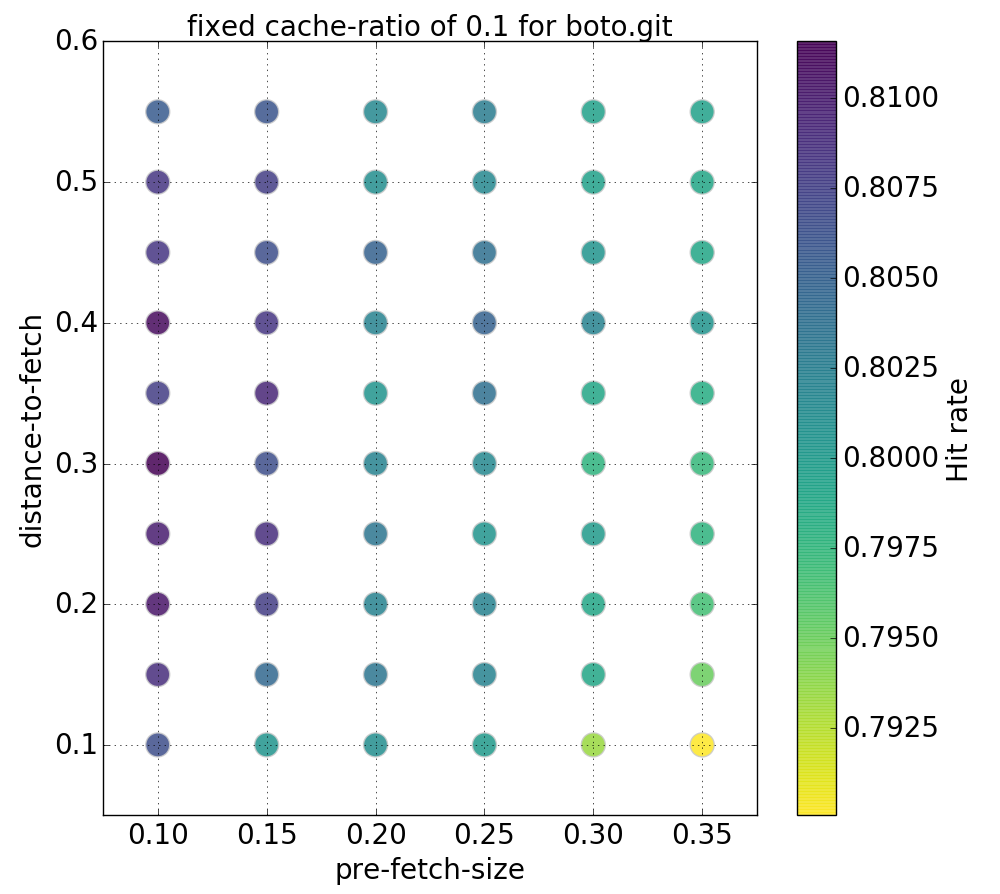
\includegraphics[width=0.5\textwidth]{fixed_cache-1.png}
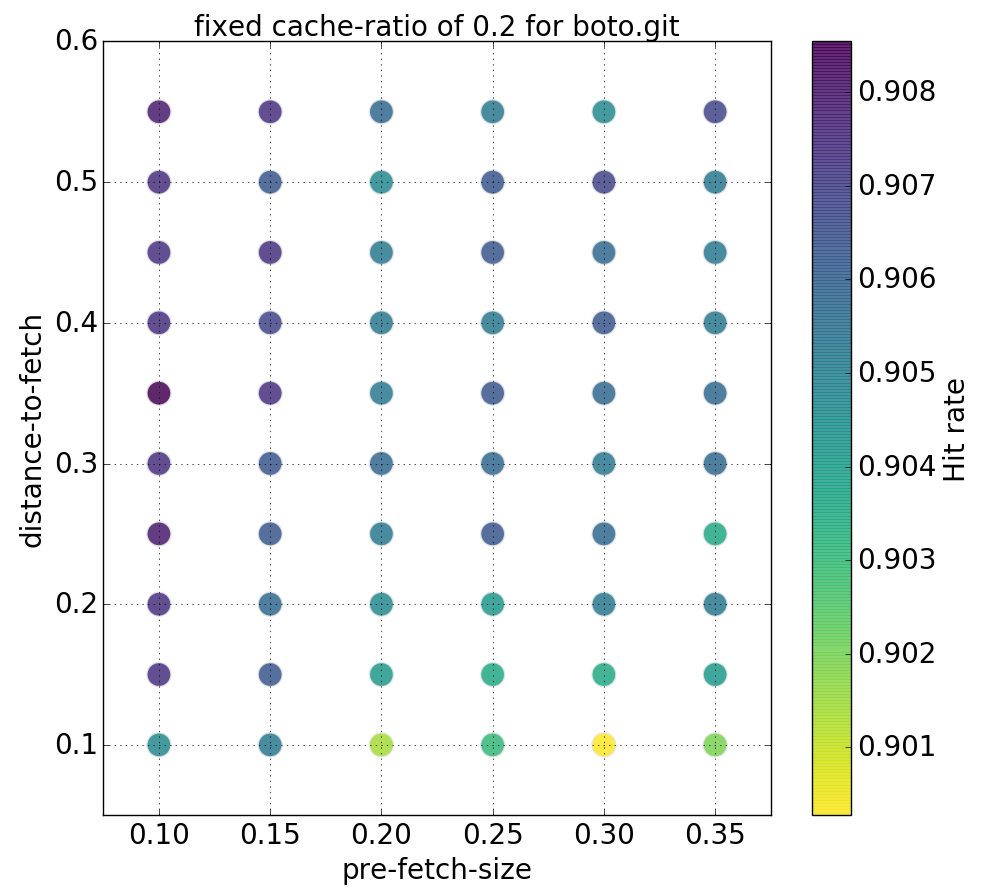
\includegraphics[width=0.5\textwidth]{fixed_cache-2.png}
\caption{Fixed cache-ratio analysis for boto.git}
\label{fig:fixed_cache}
\end{figure}
\paragraph{Finding the best pre-fetch-size and distance-to-fetch} Even though pre-fetch-size and distance-to-fetch are not the highest predictors of the cache-performance, it is still worthwhile to look at for which values of these variables is the hit-rate the biggest.
In the in figure \ref{fig:fixed_cache} we can see that for boto.git the results of a fixed-cache-ratio analysis, where we fixed the cache-ratio to 0.1 and to 0.2. The results indicate that for both we will get the best results when pre-fetch-size is low and distance-to-fetch is either 0.3 or 0.4 or 0.5. These results are in line with what was found in previous implementations\cite{FixCache}.
\paragraph{Variance in hit-rate for different variables}How big is the difference between all the plots for a given repository, at any given cache-ratio?  Figure \ref{plot_all} on the next page shows all the analyses for boto3.git and boto.git. The figure itself does not plot each and every analysis (taking all pre-fetch-size and distance-to-fetch values it would mean 15 curves), rather it plots vertical bars for each cache-ratio, where the bottom of the bar starts at the lowest hit-rate and ends at the highest hit-rate from all the analyses. That is, the bars are cover the area which was touched by any of the curves, and when a bar is taller, then the variance of hit-rates is also bigger for that repository at that cache-rate. As we can see boto3.git (which has a lot less commits than boto.git) has a higher variance in the hit-rate results, than boto.git has. The biggest difference beFor boto3.git it will be 0.158 at cache-ratio of 0.12, and for boto.git it will be 0.073 at cache-ratio of 0.02. Similarily, raspberryio.git and facebook-sdk.git would have also a high variance in this graph, so we might reason that the less commits a repository has, the bigger it's variance in the output will be. 0.076 at 0.06 for raspberryio. 0.092 at 0.16 for facebook-sdk.
\begin{figure}[t]
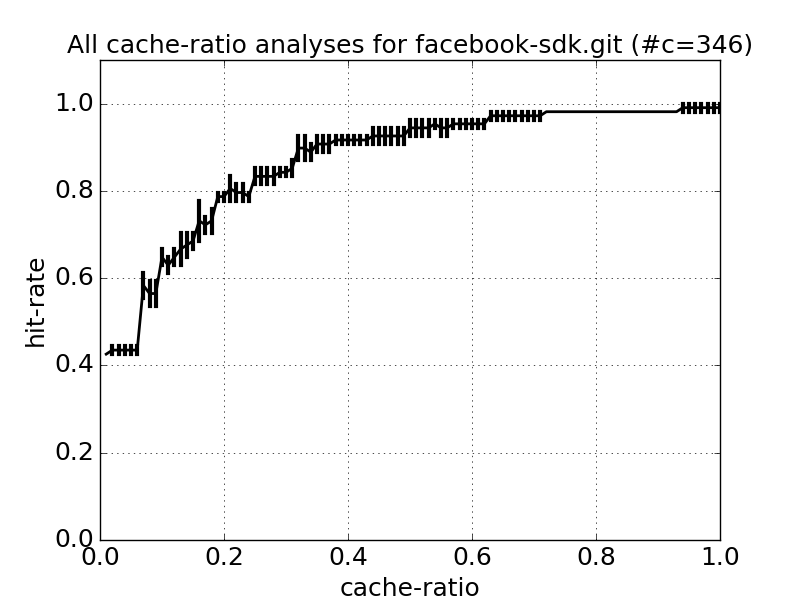
\includegraphics[width=0.5\textwidth]{plot_all-facebook-sdk.png}
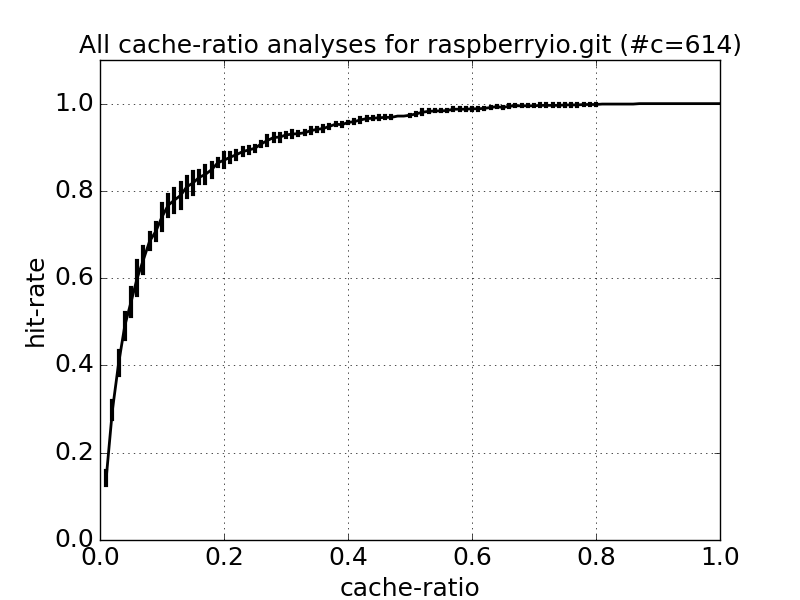
\includegraphics[width=0.5\textwidth]{plot_all-raspberryio.png}
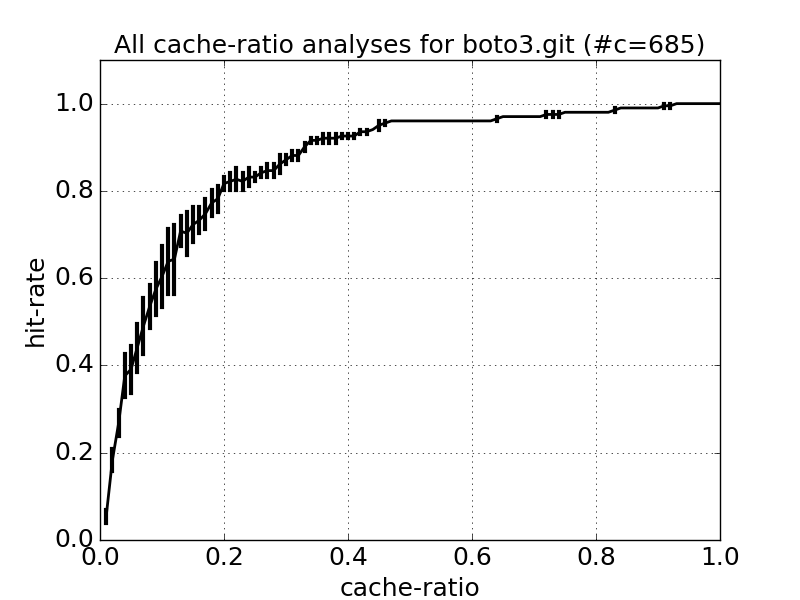
\includegraphics[width=0.5\textwidth]{plot_all-boto3.png}
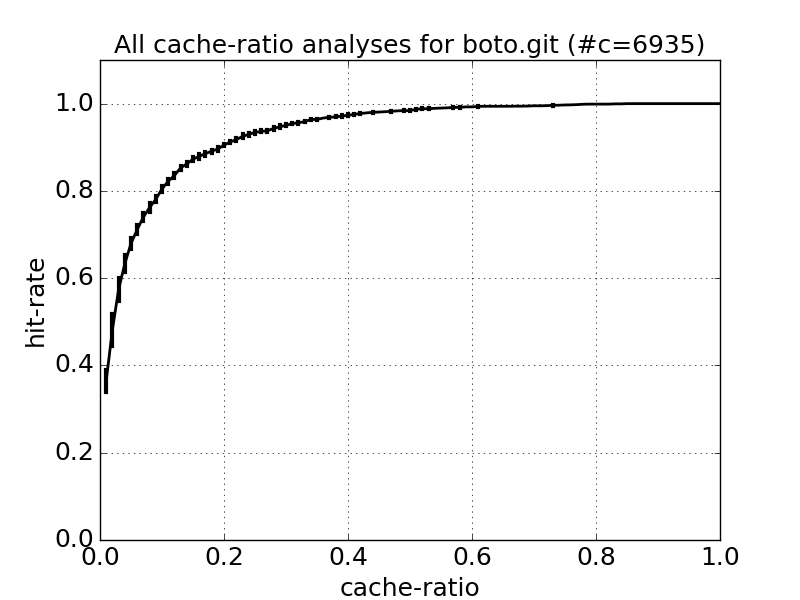
\includegraphics[width=0.5\textwidth]{plot_all-boto.png}
\caption{Showing all cache-ratio analyses for facebook-sdk.git, raspberryio.git, boto3.git and boto.git}
\label{plot_all}
\end{figure}
\paragraph{What do these results mean?} When comparing with the original paper, the results are similar (0.65-0.95 vs 0.6-0.83), although the top hit-rate boundary (0.95 for 0.1 cache-ratio) was not achieved, the highest was 0.83 for boto.git. This top boundary is reached for the cache-ratio of 0.2, which might mean that this implementation works the same for bigger cache-ratios. It is important to note that when making such a comparison one does need to remember that this implementation differs from the original in two key things: firstly, it was implemented for Git rather than Subversion and CSV and secondly it was run on Open-Source Python repositories rather than C/C++ or Java projects. 

From these results,the following points could be stated:
\begin{enumerate}
\item For a given repository R, the relationship between the number of faulty files in R and the size of R is not linear, as for a bigger R the variance decreases with variables staying the same (percentage of R's size).
\item The results found do not differ significantly from the results found in the original paper, although the same boundaries are reached for a higher cache-ratio of 0.2. Other than that, the variance between the hit-rates of different repositories is also quite big for cache-ratio of 0.1 (0.6-0.83 vs. 0.65-0.95 in the original paper), and this result seems to be connected to the number of commits in a repository (that is the history of a repository).
\item There might be several possible explanations forthese differences in cache-ratios: (a) Python programmers make more mistakes (as opposed to C/C++ or Java developers) as the language is structured differently (loose type system: duck-typing, and possibly other differences), so in general Python repositories are more vulnerable; (b) Open-source projects are more bug-prone as they are less "looked-after" and the development process is more chaotic than in organised companies and teams; (c) as Git is a distributed, de-centralized version control system, programming with the help of Git might be less structured and organised than programming with the help of Subversion or other centralised systems. Further analysis of these differences was out of the scope of this dissertation, but they definitely would be interesting to investigate further.
\item From these results we can see that \fxch{} works for Git, and also it works for Open-Source Python repositories, however the hit rate for the same parameters is slightly lower on-average.
\end{enumerate}
\subsection{Criticism}
Authors of \fxch{} claimed that after running the algorithm, our cache will contain the files which "are more likely to have a bug in the future" than others. However, they did not specify what is "future" ie. how many commits/days/weeks ahead does \fxch{} predict? To know this, we have to introduce the notion of a windowed-repository to our implementation, which will be explained later, on page \pageref{windowedrep}, and we find that \fxch{} indeed works for the first few commits in the future, but later it's accuracy drops.

Another criticism is that \fxch{} treats files as atomic entities whereas this is hardly the case. Files have several metrics on which they differ, such as LOC, or code density. If our algorithm identifies say 10\% of our file base, this 10\% might account for 20\% of all lines in the repository. This will be generally the case, as longer files are expected to have more impact and importance on our project, hence they'll have more bugs. Sadowski and colleagues \cite{Bugcache} found that even if this is the case, \fxch{} finds the files with the highest "defect densities" (files which are more bug dense: LOC/\#bugs), so the algorithm is indeed still helpful.

\section{How good is \fxch{}?}\label{windowedrep}
Evaluating over hit-rate leaves several questions open, for example "Is \fxch{} identifying files which truly have bugs in the future?", "For how many commits in the future will \fxch{} work?". When trying to answer these questions a notion of a windowed-repository was created. This means, that rather than running \fxch{} for all commits until now, we divide the commit history to a window and a horizon, and run \fxch{} on the window and we check on the horizon whether it actually worked. That is, say our window is of size 0.9, and our horizon then is 0.1, and we have 1000 commits, then we would run \fxch{} on the first 900 commits, and then check the following 100 whether it actually worked. If we look at figure \ref{fig:window_horizon} below, t0 would be at commit \#1 and tNow would be at commit \#1000. At each point in our timeline below, $c_{tX} = floor(tX)$, as the time axis below corresponds to the commit order from commit 1, to the latest commit.
\begin{figure}[h]
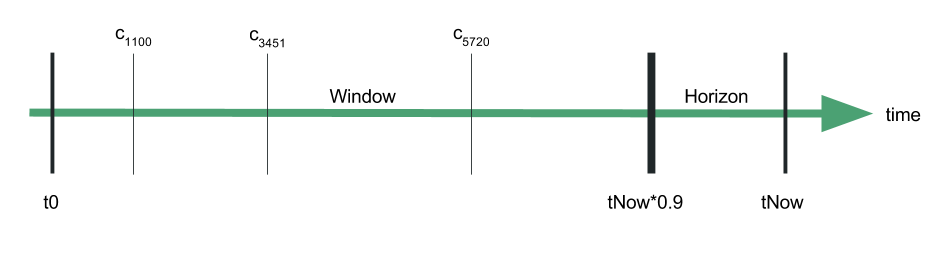
\includegraphics[width=1.0\textwidth]{window_horizon.png}
\label{fig:window_horizon}
\caption{Window and horizon presented on a timeline of commits}
\end{figure}
\subsection{Methodology}
As mentioned before, we run \fxch{} for each repository, but we stop at tNow*0.9 number of commits (the window). By default when performing such an evaluation (using \texttt{evaluation} module's \texttt{evaluate\_repository} mehtod) our default parameters are: window-ratio of 0.9, cache-ratio of 0.1, pre-fetch-size of 0.1 and distance-to-fetch of 0.5.

At the time we stop, we have some files in our cache, and this cache would be left unchanged as we walk through our horizon, lets call the set of files in the cache $CH$. Let tHStart = tNow*0.9, then at each point tX in our horizon (that is $\forall c_{tX} \in \{c_{tHStart}, \dots, c_{tNow}\}$ we can define the following two sets:
\begin{itemize}
\item Normal-file-set at tX: Files which were changed (committed) between tHStart and tX, but were not part of a bug-fixing commit in this interval. Lets call this set $NF$.
\item Faulty-file-set at tX: Files which changed in the same interval, but they were at least once changed as a part of a bug-fixing commit. Lets call this set $FF$.
\end{itemize}

From this, we can define the following properties:
\begin{itemize}
\item True-positives at tX ($TP$): The files in our cache, which indeed were faulty in [tHStart:tX]. That is $TP = FF \cap CH$.
\item False-positives at tX ($FP$): The files in our cache, which were not faulty in [tHStart:tX]. That is $FP = NF \cap CH$.
\item True-negatives at tX ($TN$): The files which are in our Normal-file-set in [tHStart:tX], and are not in our cache. That is $TN = NF \setminus CH$.
\item False-negatives at tX($FN$): The files which are in our False-file-set in [tHStart:tX], and are not in our cache. That is $FN = FF \setminus CH$.
\end{itemize}
From this we can see that all changed files in [tHStart:tX] are equal to $TP \cup FP \cup TN \cup FN$, and also that these sets are distinct.
\paragraph{Performance metrics}Following the definition of $TP$, $TN$, $FP$ and $FN$ we can define several performance metrics on which we will evaluate our windowed-repositories\cite{IR}:
\begin{enumerate}[label=(\alph*)]
\item Precision: $\frac{|TP|}{|TP| + |FP|}$
\item False discovery rate: $\frac{|FP|}{|TP| + |FP|}$
\item Negative predictive value: $\frac{|TN|}{|TN| + |FN|}$
\item False omission rate: $\frac{|FN|}{|TN| + |FN|}$
\item Recall (or sensitivity) $\frac{|TP|}{|TP| + |FN|}$ 
\item Specificity: $\frac{|TN|}{|TN| + |FP|}$
\item Accuracy: $\frac{|TP| + |TN|}{|TP| + |FP| + |TN| + |FN|}$
\item F\textsubscript{$\beta$} score: \[(1+\beta^2)*\frac{precision*recall}{(\beta^2*precision)+recall} = \frac{(1+\beta^2)*|TP|}{(1+\beta^2)*|TP| + \beta^2*|FN| + |FP|}\]

Where $\beta$ specifies whether we weight precision or recall higher.
\end{enumerate}
\subsection{Precision, recall and F\textsubscript{2} score}
\begin{wrapfigure}{r}{0.5\textwidth}
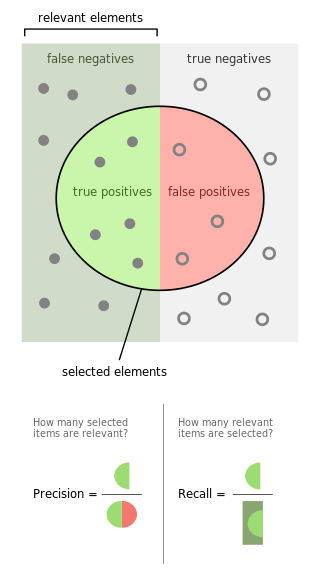
\includegraphics[width=0.48\textwidth]{Precisionrecall.png}
 \begin{minipage}{\linewidth}
    \caption[Precision and recall.]%
    {Precision and recall. Figure taken from Wikipedia\footnotemark.}
  \end{minipage}
  \label{precisionrecall}
\end{wrapfigure}
\footnotetext{https://en.wikipedia.org/wiki/Precision\_and\_recall}
Out of the metrics above, we are mostly interested in precision, recall and F\textsubscript{2} score at each bug-fixing commit in our horizon. The figure \ref{precisionrecall} on the right shows these metrics in a Venn-diagram. In this diagram the \textit{relevant elements} corresponds to fixed-files (that is ones with bugs) whereas \textit{selected elements} corresponds to files in our cache. Following this, we can define precision as the ratio of \textit{selected and relevant} files and \textit{selected but not relevant} files and recall as the ratio of \textit{selected and relevant} files and \textit{relevant} files. That is precision is tells us the percentage of files in the cache which are indeed buggy at each bug-fixing commit in our horizon while recall tells us the percentage of correctly predicted buggy files. 

As defined above the F\textsubscript{$\beta$} score weight precision and recall according to the parameter $\beta$. Since \fxch{} supposed to identify files which are `more likely to contain a bug in the future` recall should be weighted higher, as when finding buggy files it should be more important to correctly identify the biggest subset of truly faulty files than to have some false-positives, therefore F\textsubscript{2} score will be used for evaluation.
\subsection{Results}
\subsubsection{Evaluating boto.git}
\begin{figure}[ht!]
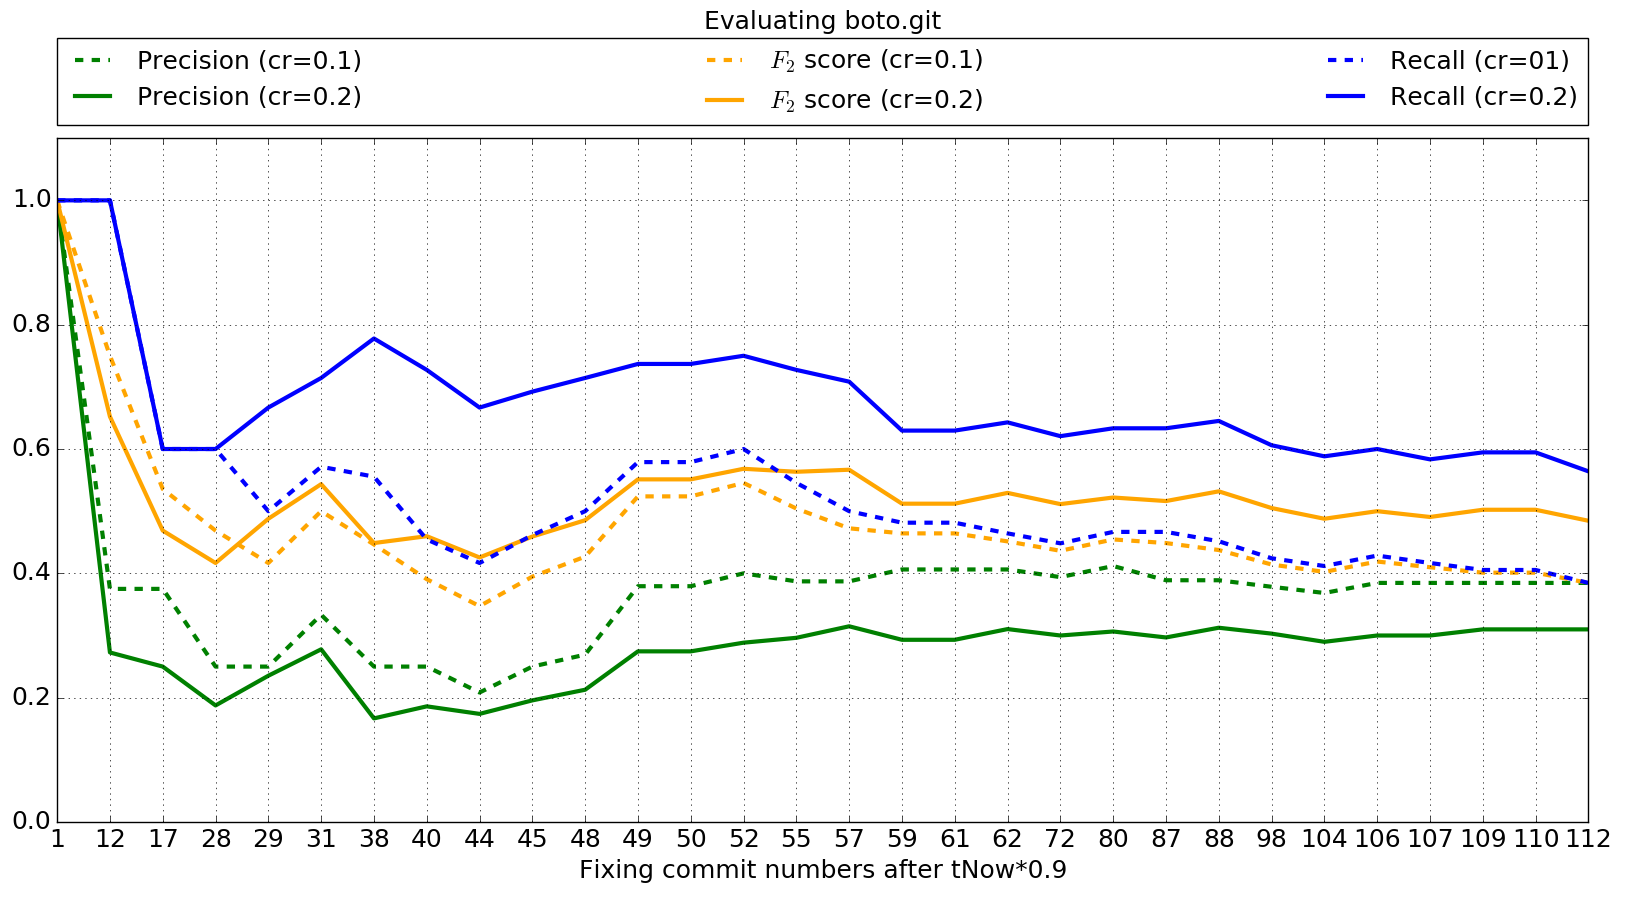
\includegraphics[width=1.0\textwidth]{evaluating_boto.png}
\caption[Evaluating boto.git: recall, precision and $F_2$ score]{Evaluating boto.git with precision, recall and F\textsubscript{2} score for the first 30 commits in the horizon after tNow*0.9.}
\label{evaluating_boto}
\end{figure}
Figure \ref{evaluating_boto} shows precision, $F_2$ score and recall for the first 30 fixing commit in the horizon for boto.git (at cache-ratio of 0.1 and 0.2), which at the time of evaluation has 6935 commits. For cache-ratio of 0.2 we can see that for the first fixing-commit in the horizon (that is for $c_1$) all the metrics are equal to 1.0. That is our algorithm identified buggy files fixed at $c_1$ correctly. However, at the second fixing commit, there is a massive drop in all three metrics, except for recall, when this drop occurs between $c_{12}$ and $c_{17}$ rather than between $c_1$ and $c_{12}$. If we look at recall, it always stays above 0.6 (except for the last few commits), that is we will identify at least 60\% of the truly buggy files. Furthermore, after the sudden drop, it will have it's peak of 0.78 at $c_{38}$, after which it will continue to drop.

Recall at cache-ratio of 0.1 is lower or equal to the recall at 0.2, which is expected. However, precision is higher, which is due to the higher number of false-positives identified when having a bigger cache.

From this figure, we can deduce that for boto.git \fxch{} does only perform well for the first two commits in terms of recall, and does poorly afterwards (except the peak at $c_{38}$; similarly it only works for the first commit for the other two metrics, after which precision and $F_2$ score will also drop. This means that in this case \fxch{} should not be used as a long-term bug-prediction technique, but rather as a source for finding recently introduced bugs. Also, we can see that the performance is better with cache-ratio of 0.2.
\subsubsection{Evaluating django.git}
\begin{figure}[ht!]
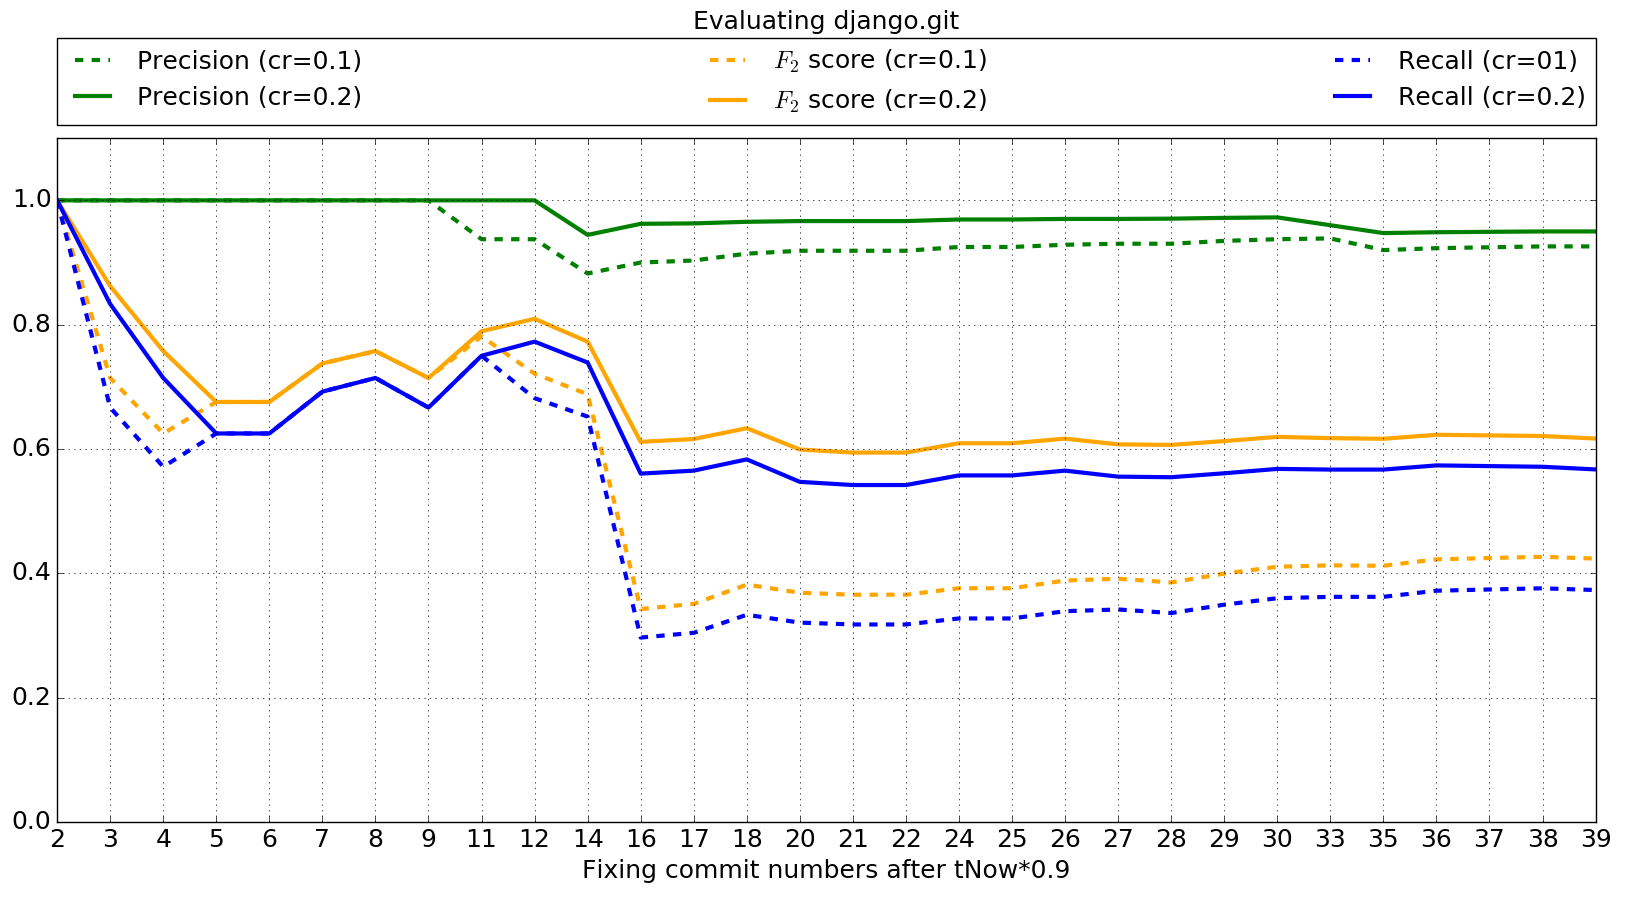
\includegraphics[width=1.0\textwidth]{evaluating_django.png}
\caption[Evaluating django.git: recall, precision and $F_2$ score]{Evaluating django.git with precision, recall and F\textsubscript{2} score for the first 30 commits in the horizon after tNow*0.9.}
\label{evaluating_django}
\end{figure}
Figure \ref{evaluating_django} shows the same data as \ref{evaluating_boto} but this time for django.git, which has 22352 commits at the time of the evaluation. Also, a difference to observe is that nearly every commit in the horizon looked at is a fixing-commit (as we arrive at commit \#39 which is the 30\textsuperscript{th} fixing-commit), that is fixes occur much more frequently. This is likely due to the fact that django.git is already a complete product, and all these fixing-commits are responses to issues reported by users rather than by the developers themselves. That is the implementation of django.git is finished (at least on the master branch) and hence nearly all the commits are fixing ones. 

Again as with figure \ref{evaluating_boto} the metrics are higher for cache-ratio of 0.2 (even for precision this time). However, the difference between cache-ratios is much bigger for the $F_2$ score after the drop happens (here at $c_{12}$). We can see that the difference between $F_2$ scores for cache-ratio of 0.1 and 0.2 will be at least 0.2 after this point. This difference was never as dramatic in figure \ref{evaluating_boto}.

Another key difference between this figure and figure \ref{evaluating_boto}: precision stays high for all the commits. That is, if a file is identified as a buggy-file here, it is likely to indeed be buggy: our cache indeed has faulty files in it. Other than this, recall also drops after the first two commits, after which it also climbs back to a peak at around 0.78 (here at $c_{12}$), and after this peak it will drop below 0.6, so it is slightly worse than recall for boto.git.
\addcontentsline{toc}{chapter}{Bibliography}
\bibliography{refs}
\end{document}
